%%
%% Copyright (c) 2018-2019 Weitian LI <liweitianux@sjtu.edu.cn>
%% Creative Commons BY 4.0
%%

\chapter{基于深度学习的再电离信号分离新算法}
\label{chap:cdae}

为了能够从强烈的前景干扰中分离出微弱的 EoR 信号,
传统的\ac{fg-rm}方法都依赖于一个关键的前提:
前景干扰具有非常光滑的频谱,而 EoR 信号沿频率维度发生剧烈变化,
两者具有显著不同的频谱结构,从而能够被有效地分离开 \cite{morales2010,chapman2016}.
然而,在实际情况中,未分辨的或者未完全扣除的干扰源在干涉阵列的波束效应的影响下,
会在频率维度产生震荡形式的辐射,破坏前景频谱的光滑性 \cite{liu2009ps}.
这会显著削弱前景干扰与 EoR 信号的可分性,
导致传统\ac{fg-rm}方法的效果大打折扣甚至失效,
因此需要研发能够克服波束效应的 EoR 信号分离新算法.


%=====================================================================
\section{波束的频率依赖效应}
\label{sec:beam-effect}

\begin{figure}[htp]
  \centering
  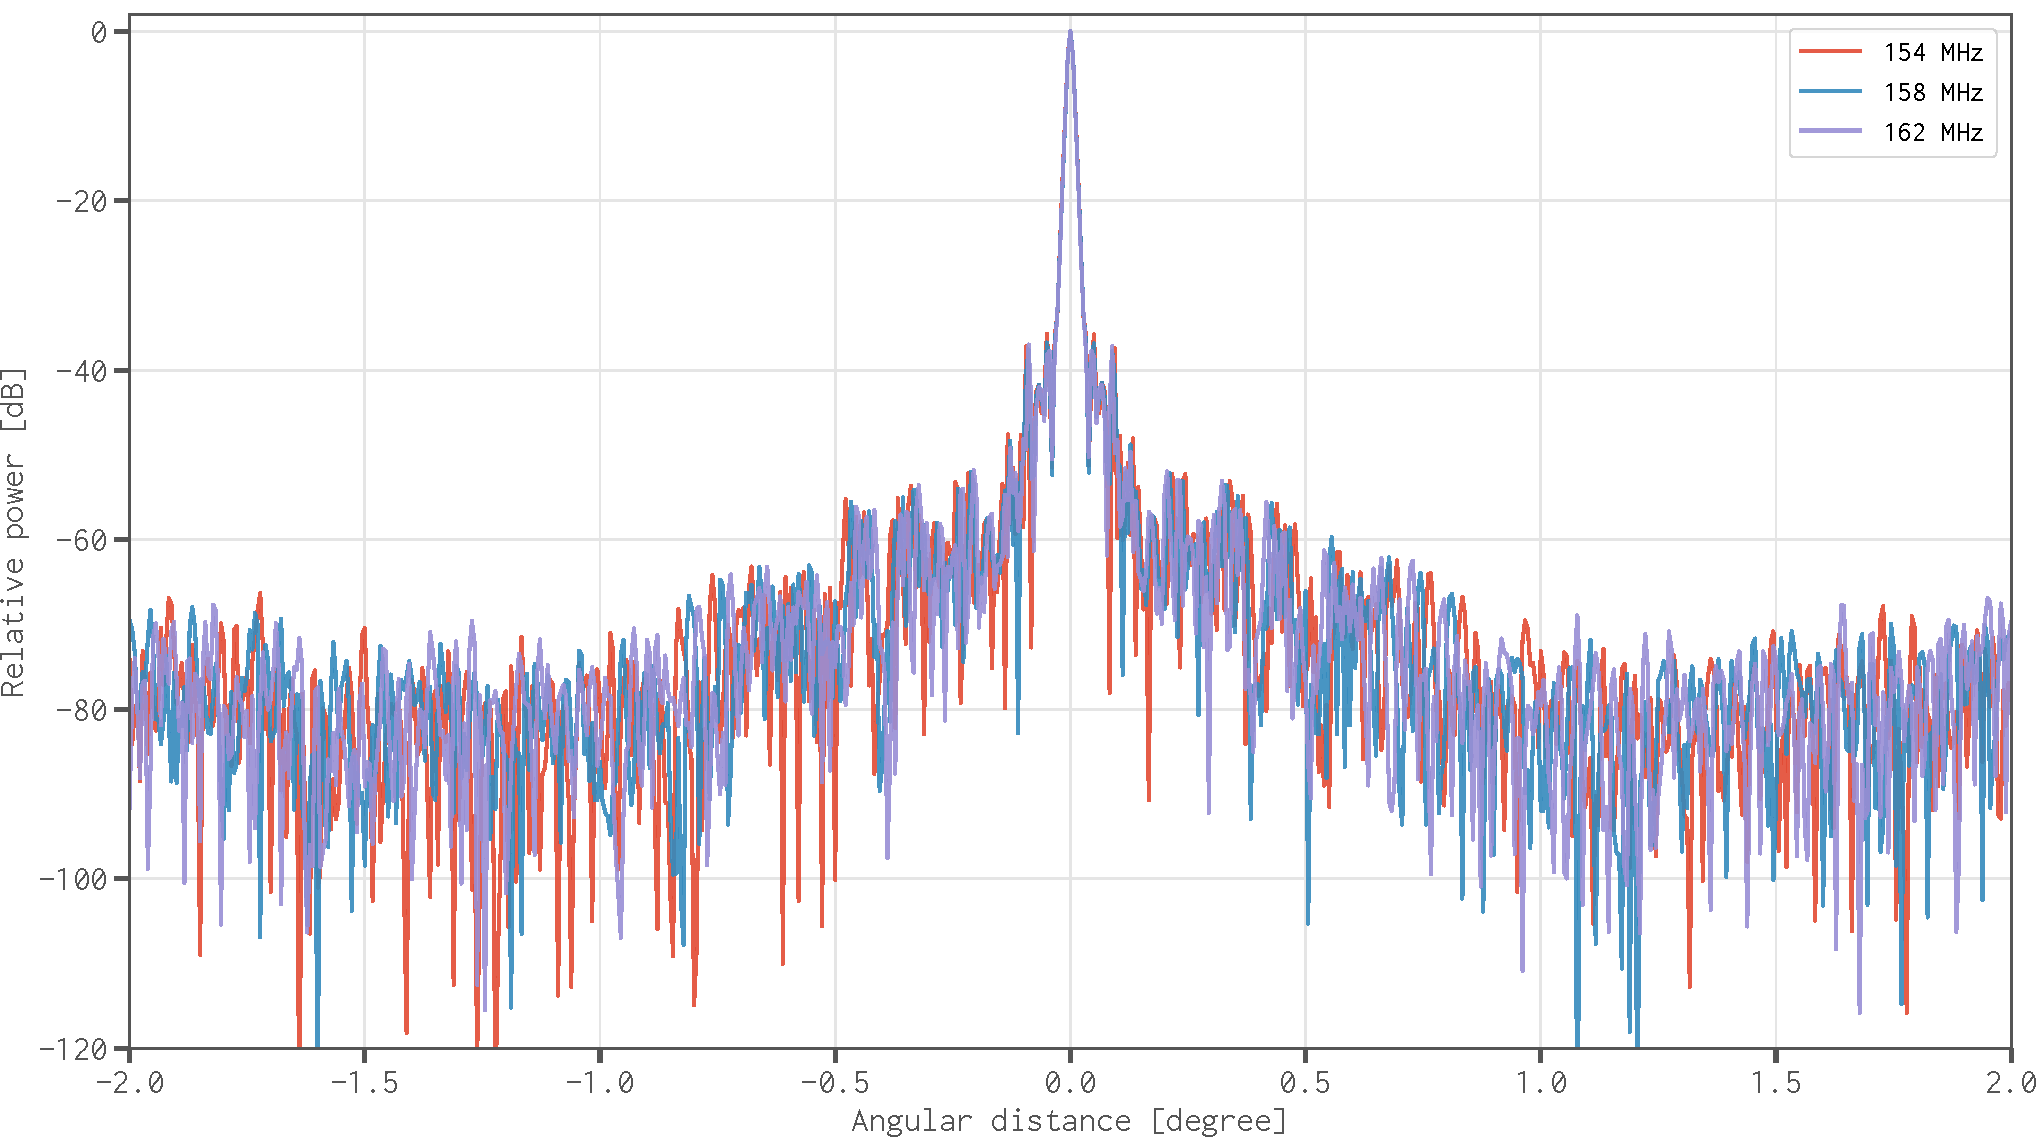
\includegraphics[width=\textwidth]{SKA1-low-psf}
  \bicaption[模拟的 SKA1-Low 综合波束]{%
    在 154、158 和 162 MHz 处模拟的 SKA1-Low \acs*{beam-synthesized}.
    积分时间为 \SI{6}{\hour}.
  }{%
    The simulated synthesized beams of SKA1-Low at 154, 158, and 162 MHz.
    The integration time is \SI{6}{\hour}.
  }
  \label{fig:ska-psf}
\end{figure}

一个干涉阵列拥有的\ac{baseline}的数目和长度均是有限的,
在观测中能实现的 $uv$ 覆盖也是有限而且不完备的 (\autoref{sec:uv-coverage}),
因此,干涉阵列的\ac{beam-synthesized}的形状非常复杂.
如\autoref{fig:ska-psf} 所示,
除了中间一个很窄的\ac{mainlobe},\ac{beam-synthesized}还包含一系列\ac{sidelobe}.
这些\ac{sidelobe}的数量非常多,相对幅度约为 \numrange{0.01}{0.1}\%,
一直延伸到远超出视场的位置.
另见 \citeay{liu2009ps} 的图 1 和图 3.

另一方面,\ac{beam-synthesized}的形状还依赖于观测频率.
\ac{sidelobe}的位置 $\theta$ 会随着频率 $\nu$ 的增大而向中间移动,
即 $\theta \propto \nu^{-1}$.
因此,一个干扰源在视场中所产生的辐射的位置也随频率而变化.
由于仪器的热噪声水平、成像的天区大小、CLEAN 的深度等因素的限制,
视场中总是存在一批未分辨的以及未完全扣除而残留的干扰源.
由这些干扰源的辐射综合而成的前景干扰,
在频率维度将出现类似\ac{beam-synthesized}的\ac{sidelobe}形状的起伏.
这将破坏前景辐射的频谱光滑性,使得前景干扰具有类似 EoR 信号的小尺度频谱结构,
导致传统\ac{fg-rm}方法无法有效地将两者区分开.
另见 \citeay{liu2009ps} \S\,1.


%=====================================================================
\section{基于深度学习的新算法}

鉴于\ac{beam-synthesized}的形状非常复杂,并且随频率和位置而变化,
即使付出昂贵的计算代价,
为传统\ac{fg-rm}方法手工打造一个用于克服上述波束效应的模型仍然是非常困难的
\cite{lochner2015}.
此外,SKA1-Low 等大型干涉阵列的海量数据的处理已经成为一个重要的瓶颈 (ref???),
所以采用传统\ac{fg-rm}方法并建模克服波束效应在实际应用中几乎不可行.
相比于传统方法,\ac{dl}方法能够自动地从数据中汲取信息用来优化模型;
一旦训练好模型,使用该模型则变得非常高效;
方法的灵活性高,只需要使用合适的数据重新训练,便可以将方法运用于其他望远镜.
因此,基于\ac{dl}研发能够克服波束效应的 EoR 信号分离算法更具有可行性和吸引力
\cite{herbel2018,vafaeiSadr2019}.

\begin{figure}[htp]
  \centering
  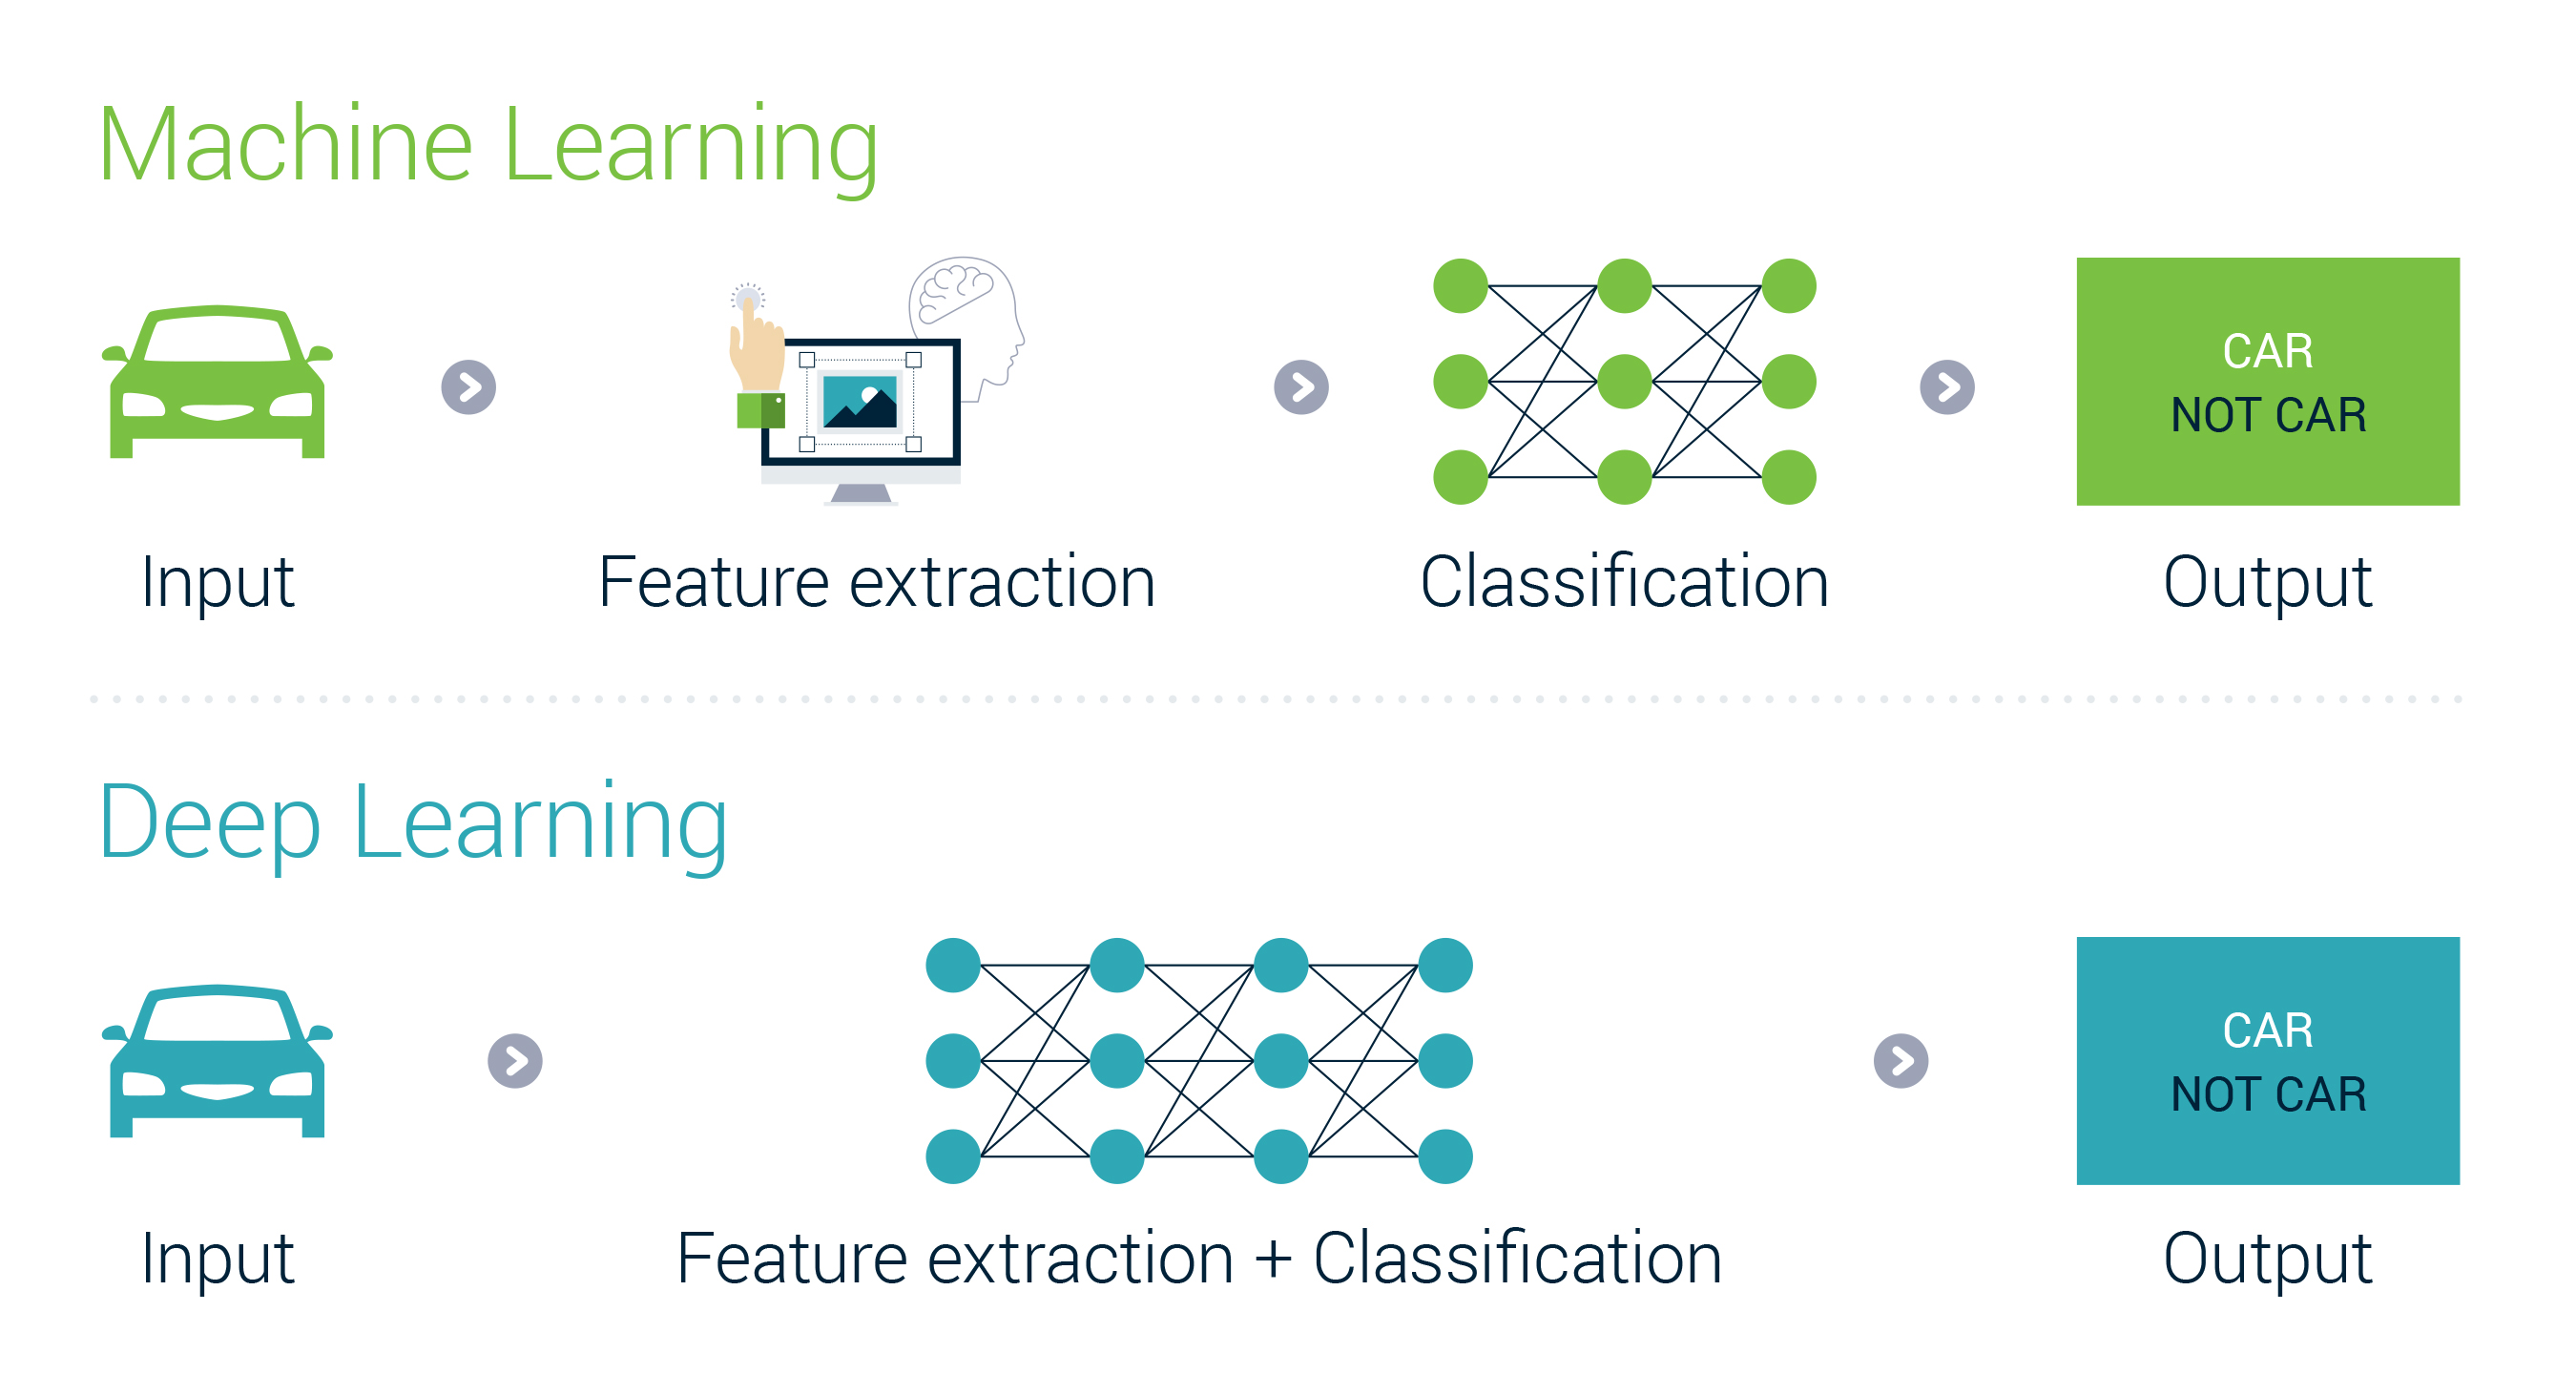
\includegraphics[width=\textwidth]{ml-vs-dl}
  \bicaption[机器学习和深度学习之间的主要区别]{%
    机器学习和深度学习之间的主要区别.
    深度学习拥有\acs*{fx}的能力,而不必手工设计需要从数据中提取的特征.
  }{%
    The main difference between machine learning and deep learning.
    The feature extraction is an integral part of the deep learning;
    therefore, there is no need to craft the features to be extracted
    from the data.
    \\来源/Credit:
    Jochem Grietens,
    \url{https://verhaert.com/difference-machine-learning-deep-learning/},
    (2019-04-25)
  }
  \label{fig:ml-dl}
\end{figure}

\ac{dl}是\ac{ml}的一个子集,同时后者又是\ac{ai}的一个子集.
\ac{ai}起始于上世纪 50 年代,该领域的开创人之一 John McCarthy 将\ac{ai}定义为
\enquote{制造智能机器的科学和工程} \cite{mcCarthy2007}.
早期的\ac{ai}系统完全基于一整套规则,而这些规则需要明确地由人来定义和实现 (ref???).
\ac{ml}是另一条实现\ac{ai}的途径,通过让机器从数据中学习并调整自身模型,
达到智能化判断或预测的目的.
利用该方法,我们只需要设计机器需要从数据中提取的特征以及相应的学习策略,
而不需要编写每一条具体的规则,有效地减轻了开发\ac{ai}系统的负担 (ref???).
\ac{dl}是\ac{ml}中的一类技术,让机器拥有了\ac{fx}的能力,
进一步降低了开发先进的\ac{ai}系统的难度,极大地拓展了\ac{ai}的应用范围 (ref???).
\autoref{fig:ml-dl} 示意了\ac{ml}和\ac{dl}之间的主要区别.

近十多年以来,\ac{dl}发展迅猛,已经被应用到诸多领域并取得了一系列突破性成果,
详见 \citeay{leCun2015} 综述文.
\ac{dl}方法包括多种\ac{nn} \cite{bengio2009,leCun2015,schmidhuber2015},
比如\ac{dnn}、\ac{cnn}、\ac{rnn}、\ac{ae}.
其中,\ac{ae}能够以\ac{unsupervised}的方式从输入数据中发掘有用的特征,
从而学习得到输入数据的一个有效\ac{representation} \cite{bourlard1988}.
因此,\ac{ae}经常被用于数据的\ac{dim-reduction}\cite{hinton2006,wang2014}
和\ac{denoising}\cite{xie2012,lu2013,bengio2013}.
在\ac{ae}的诸多变种中,\ac{cdae}尤其擅长于发掘数据中的抽象、细微的特征 \cite{du2017},
并且已经被成功地用于微弱\ac{gw}信号的\ac{denoising}\cite{shen2017}、
单声道音源的分离\cite{grais2017}、等等.

这些应用说明了 \ac{cdae} 具有从高度时变 (temporal-variable)
的数据中提取微弱信号的出色能力,
因此,值得尝试将 \ac{cdae} 应用于 EoR 信号的分离.
尽管待分离的 EoR 信号的\ac{snr}比上述应用中的情况更低,
但是 EoR 信号、前景辐射以及望远镜的波束效应都是稳定或近似稳定的.

%---------------------------------------------------------------------
\subsection{卷积去噪自编码器}
\label{sec:cdae}

\begin{figure}[htp]
  \centering
  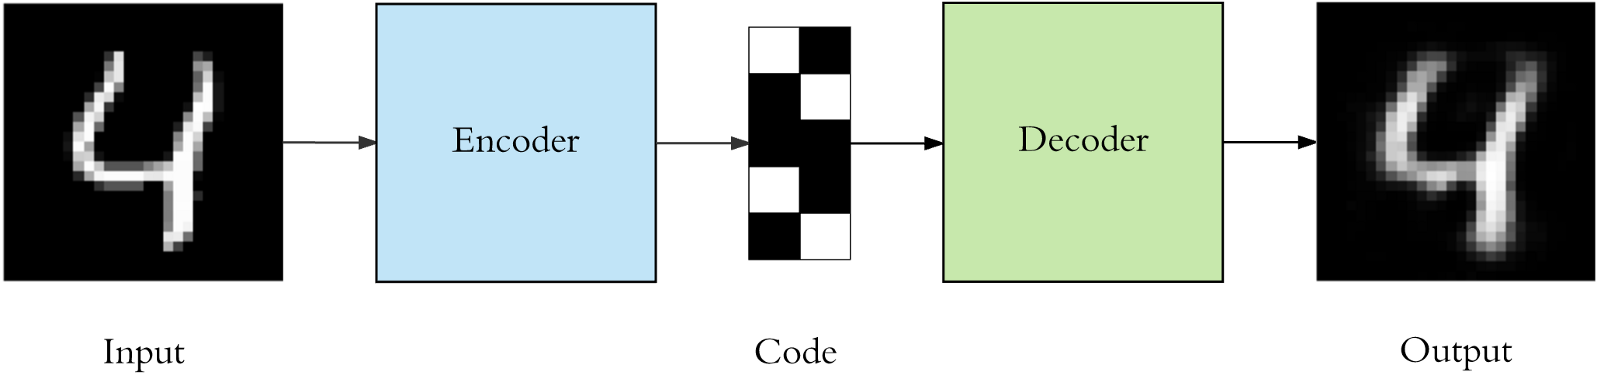
\includegraphics[width=0.8\textwidth]{autoencoder}
  \bicaption[自编码器的示意图]{%
    \acs*{ae}的示意图.
  }{%
    Diagram of an autoencoder.
    \\来源/Credit:
    Arden Dertat,
    \url{https://towardsdatascience.com/applied-deep-learning-part-3-autoencoders-1c083af4d798},
    (2019-04-25)
  }
  \label{fig:autoencoder}
\end{figure}

\emph{\ac{ae}}由\ac{encoder}和\ac{decoder}两部分组成,
其中\ac{encoder}将输入信号 $\B{x}$ 映射成一个内部\ac{code} $\B{h}$,
可表示为 $\B{h} = f(\B{x})$;
\ac{decoder}则尝试从\ac{code} $\B{h}$ 重建原输入信号,
可表示为 $\B{r} = g(\B{h})$;
如\autoref{fig:autoencoder} 所示.
因为我们将在频率维度对天空像素点逐个进行 EoR 信号的分离,
所以,输入信号 $\B{x}$ 表示一个天空像素点的频谱,
$\B{x}$、$\B{h}$ 和 $\B{r}$ 在本工作中均为一维矢量.
通过对\ac{code} $\B{h}$ 施加一定的约束(如限制其维度或稀疏性),
同时训练\ac{ae}使得重建信号 $\B{r}$ 与输入信号 $\B{x}$
之间的\ac{loss} $L(\B{r}, \,\B{x})$ 达到最小,
则\ac{ae}所学习到的\ac{code}将能有效地表示输入信号.
详见 \citeay{goodfellow2016}, 第 14 章.

\ac{ae}所学到的\ac{representation}的质量直接决定了\ac{ae}的性能.
为了促使\ac{ae}学习一个更好的\ac{representation},
\citeay{vincent2008} 和 \citeay{vincent2010}
基于\enquote{\ac{denoising}准则}提出了一种全新的训练策略:
首先人为地损坏(比如加入噪声)原始输入信号 $\B{x}$,
得到受损信号 $\B{x}'$ 并输入\ac{ae}进行训练,
使其重建信号 $\B{r}$ 尽可能地恢复原始输入信号 $\B{x}$,
即最小化\ac{loss} $L(\B{r}, \,\B{x})$.
这个\ac{denoising}过程迫使\ac{ae}发掘原始输入信号 $\B{x}$
中那些对准确重建起关键作用的稳健特征.
使用该\ac{denoising}准则训练的\ac{ae}也被称为\emph{\ac{dae}}.

\begin{figure}[htp]
  \centering
  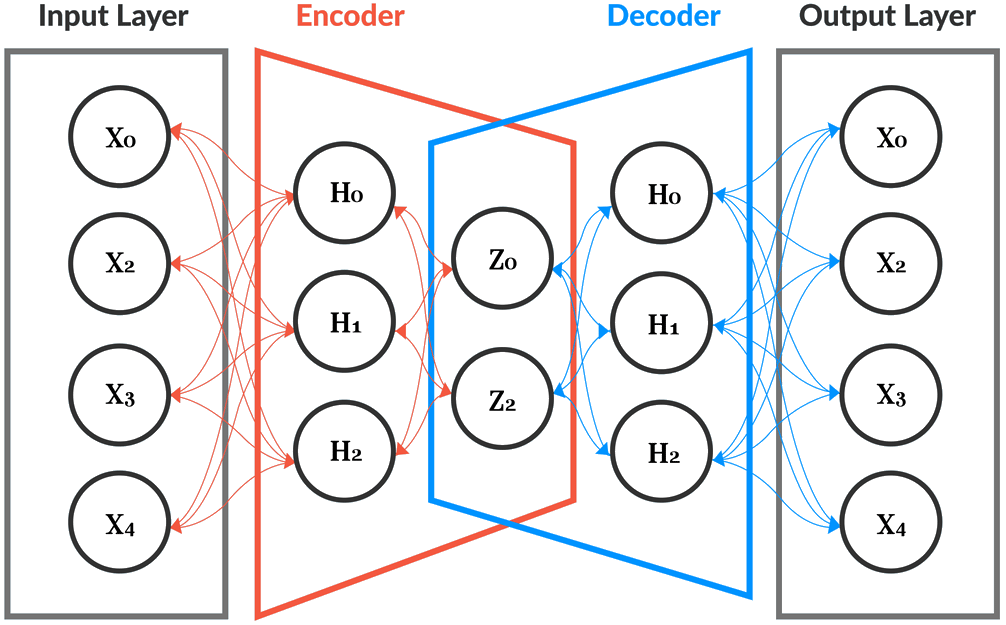
\includegraphics[width=0.6\textwidth]{autoencoder-fc}
  \bicaption[使用全连接层的经典自编码器的示意图]{%
    使用\acs*{fc}层的经典\acs*{ae}的示意图.
    \acs*{fc}层的每个\acs*{neuron}都与上一层的所有的\acs*{neuron}相连.
  }{%
    Diagram of a classic autoencoder that uses fully connected layers.
    Every neuron in a fully connected layer is connected to all neurons
    in the previous layer.
    \\来源/Credit:
    Trix Genota,
    \url{https://medium.com/@abien.agarap/implementing-an-autoencoder-in-tensorflow-2-0-5e86126e9f7},
    (2019-04-26)
  }
  \label{fig:autoencoder-fc}
\end{figure}

\begin{figure}[htp]
  \centering
  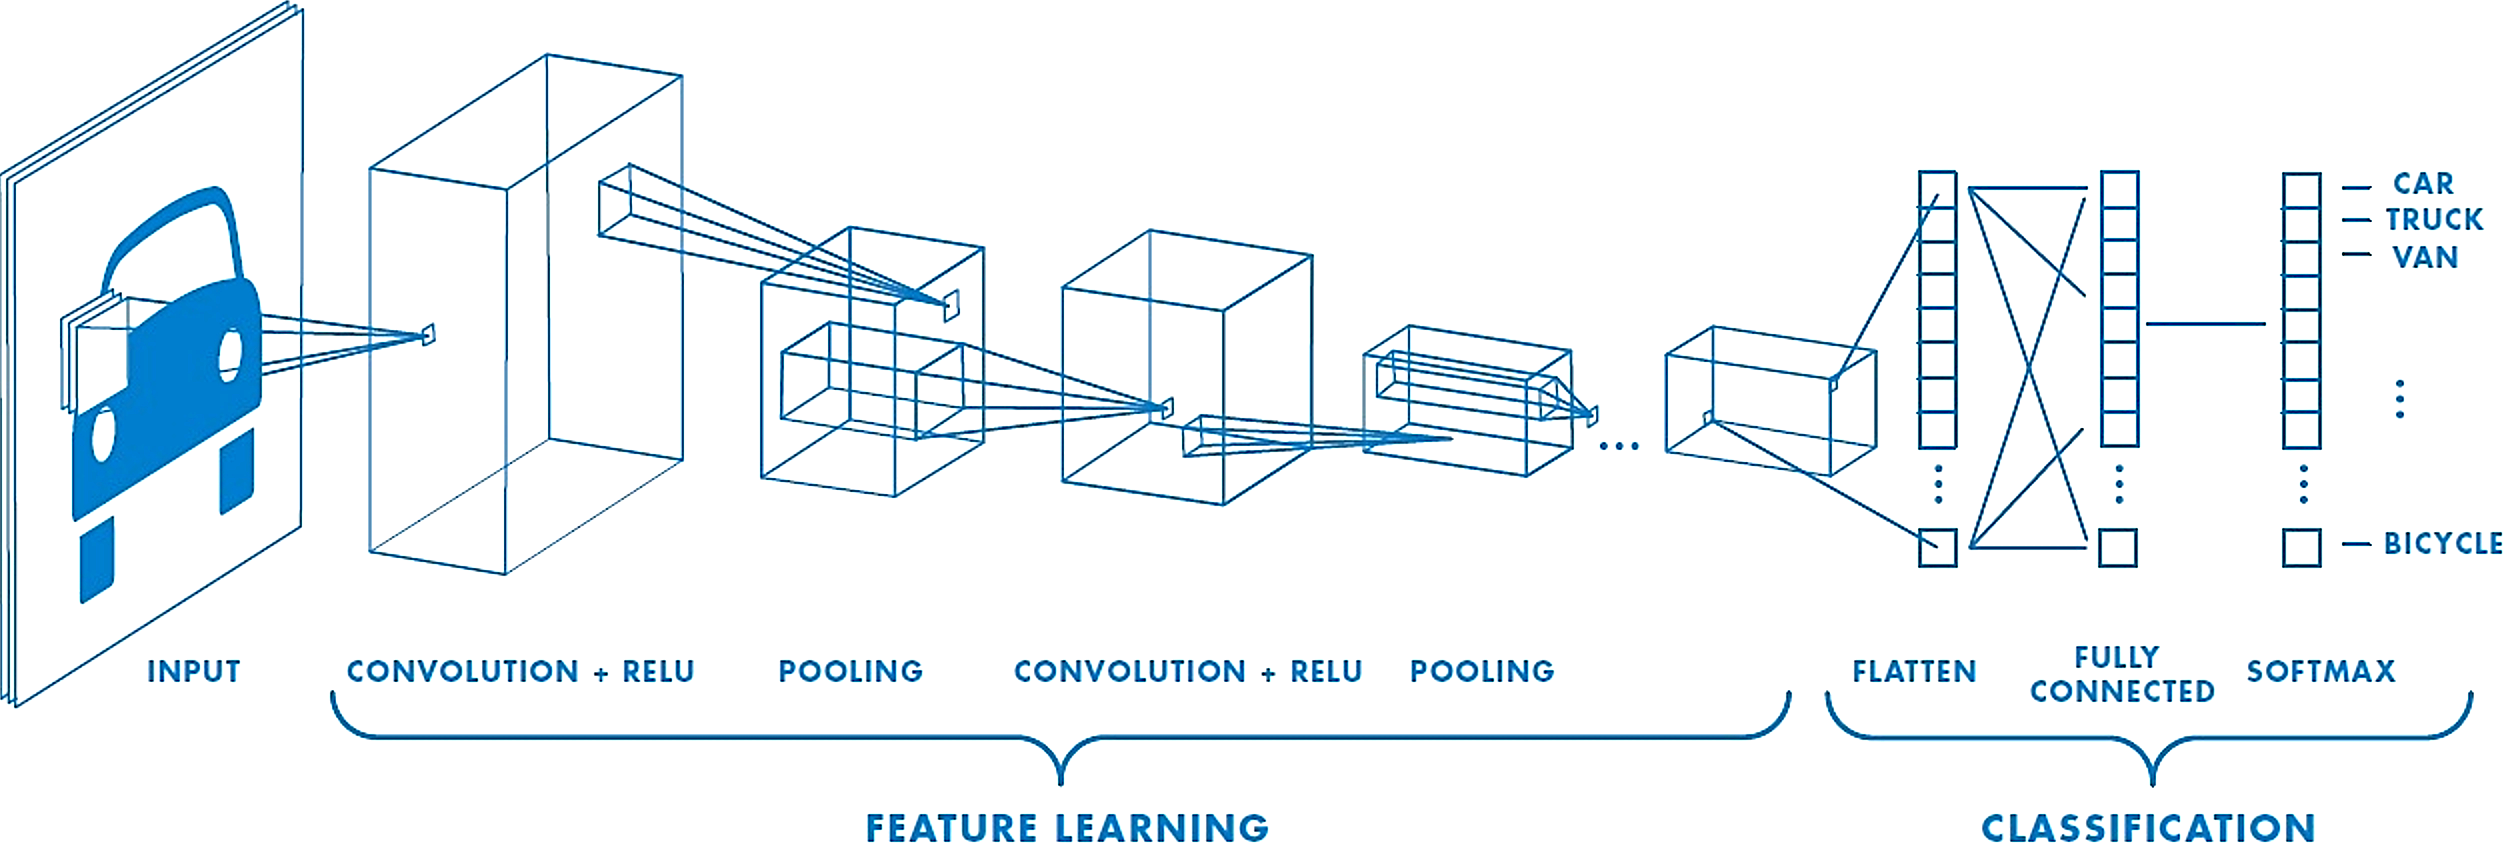
\includegraphics[width=\textwidth]{cnn}
  \bicaption[卷积神经网络的示意图]{%
    卷积神经网络的示意图,一般包括多个卷积层,
    每个卷积层由一组小尺寸\acs*{filter}构成,
    每个\acs*{filter}在数据的所有位置共享其参数.
  }{%
    Diagram of a convolutional neural network,
    which includes several convolutional layers.
    A convolutional layer consists of a set of small filters,
    each of which shares its weights among all locations in the data.
    \\来源/Credit:
    Sumit Saha,
    \url{https://towardsdatascience.com/a-comprehensive-guide-to-convolutional-neural-networks-the-eli5-way-3bd2b1164a53},
    (2019-04-26)
  }
  \label{fig:cnn}
\end{figure}

经典\ac{ae}由多个\ac{fc}层构成,其中每个\ac{neuron}都与上一层的所有\ac{neuron}相连,
如\autoref{fig:autoencoder-fc} 所示.
这种设计使\ac{ae}的参数数目随层数呈指数级增长,难以构建很深的网络.
此外,使用\ac{fc}层提取的特征是全局性的,
所以\ac{fc}层不适合用来学习输入数据中的局部特征(如图像中的文字、物体等),
而这些局部特征通常包含了数据的关键信息 \cite{masci2011}.
在另一方面,\ac{cnn}则使用多个卷积层来提取数据中的特征,如\autoref{fig:cnn} 所示.
每个卷积层由一组小尺寸(大小通常为 3、5、7)\ac{filter}构成,
每个\ac{filter}的权重参数不随数据的位置而变化.
这样,卷积层非常适合于提取数据中的局部特征 \cite{leCun1998},
同时有效地减少了参数数目.
\ac{cnn} 的参数数目通常约为类似的\ac{fc}\ac{nn}的 1\% 或更少 \cite{grais2017},
所以 \ac{cnn} 更容易训练,消耗的资源(如内存和时间)也更少.
另外,多个卷积层可以很容易地堆叠起来;
在前一层所提取的特征的基础上,更复杂、更抽象的特征能够从数据中提取出来.
这种技术推动我们设计出极深(几十层甚至上百层)、极富表达力的 \ac{cnn},
并且这些 \ac{cnn} 在图像分类及相关领域有着非凡的表现
\cite{krizhevsky2012,simonyan2014,szegedy2015,ma2019}.

\emph{\ac{cdae}} 是使用了多个卷积层而非\ac{fc}层的\ac{dae},
因此拥有和 \ac{cnn} 一样强大的\ac{fx}能力.
如此一来,\ac{cdae} 有能力从输入数据中学习一个更好的\ac{representation},
从而拥有更强的\ac{denoising}能力,能够重建即使严重受损的信号 \cite{du2017}.
所以,\ac{cdae} 非常适合用来发掘 EoR 信号和前景辐射之间的复杂区别,
进而实现两者的准确分离.

%---------------------------------------------------------------------
\subsection{网络架构}
\label{sec:architecture}

\begin{figure}[htp]
  \centering
  % Credit: https://tex.stackexchange.com/a/201120
  \rotatebox[origin=c]{90}{%
    \begin{minipage}{0.99\textheight}
      \centering
      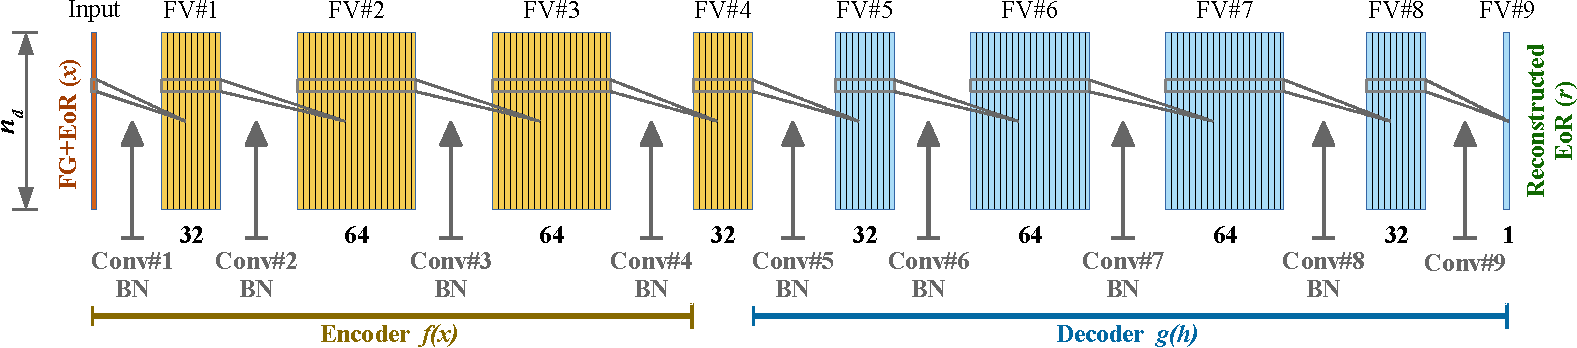
\includegraphics[width=\linewidth]{cdae-network-crop}
      \bicaption[CDAE 网络架构示意图]{%
        本文所提出的 CDAE 网络架构示意图,
        由一个四层的\acs*{encoder}和一个五层的\acs*{decoder}组成.
        黄色和蓝色方框分别表示\acs*{encoder}和\acs*{decoder}输出的\acs*{fv} (FV),
        方框下方的数字表示相应的卷积层所包含\acs*{filter}的数目.
        除了最后一层,其他层均使用了\acs*{batch-norm} (BN) 技术.
      }{%
        The architecture of the proposed CDAE that consists of a
        four-layer encoder and a five-layer decoder.
        The yellow and blue boxes represent the feature vectors (FV)
        generated by the encoder and decoder layers, respectively.
        The numbers marked below the boxes are the number of filters in
        the corresponding convolutional layers.
        The batch normalization (BN) technique is applied to all layers
        except for the last layer.
      }
      \label{fig:cdae-network}
    \end{minipage}
  }
\end{figure}

\ac{ae}的\ac{encoder}和\ac{decoder}部分均包含多个卷积层.
因为我们关注于\ac{ae}的\ac{fx}能力和\ac{denoising}能力,
而不关心所得\ac{code} $\B{h}$ 的具体形式,
所以\ac{encoder}和\ac{decoder}之间并没有明确的界线.
设第 $l$ 个卷积层包含 $m_l$ 个\ac{filter}
$\left(\left\{ k_{i}^{(l)} \right\};\, i = 1, 2, \cdots, m_l \right)$,
其中每个\ac{filter} $k_{i}^{(l)}$ 卷积前一层的输出,
得到一个\ac{fv} $\B{v}_{i}^{(l)}$:
\begin{equation}
  \label{eq:conv}
  \B{v}_{i}^{(l)} = \phi^{(l)} \left( \sum_{j=1}^{m_{l-1}}
    \B{v}_{j}^{(l-1)} * W_i^{(l)} + b_i^{(l)} \right) ,
    \quad i = 1, 2, \cdots, m_{l} ,
\end{equation}
其中
$W_i^{(l)}$ 和 $b_i^{(l)}$ 分别是\ac{filter} $k_{i}^{(l)}$
的权重和\ac{bias}参数,
$\phi^{(l)}(\cdot)$ 是当前第 $l$ 层的\ac{f-activation},
$\B{v}_{j}^{(l-1)}$ 为前一层的输出,
\enquote{$*$} 表示卷积运算.
于是,第 $l$ 层的输出为该层所有\ac{filter}的\ac{fv}所构成的集合
$\left(\left\{ \B{v}_{i}^{(l)} \right\};\, i = 1, 2, \cdots, m_l \right)$.

我们遵循\ac{dl}的推荐做法\cite{geron2017,suganuma2018} 来设计 \ac{cdae} 的架构.
具体而言,所有卷积层的\ac{filter}的尺寸为 3,
并且使用\ac{elu}作为\ac{f-activation} $\phi^{(l)}(\cdot)$ \cite{clevert2016},
除了最后一层(即\ac{ae}的输出层)的\ac{f-activation}为\ac{f-tanh} \enquote{tanh}
(参见 \autoref{sec:preprocessing}).
此外,除了最后的输出层,其他层均使用了\ac{batch-norm}技术 \cite{ioffe2015}.
该技术不仅可以加快训练速度,提高模型的准确率,
还能作为一个\ac{regularizer}预防\ac{overfitting} \cite{geron2017}.

为了确定 \ac{cdae} 的卷积层数目以及每个卷积层的\ac{filter}个数,
我们构建了许多个包含不同数量的卷积层和\ac{filter}的 \ac{cdae},
然后评估这些 \ac{cdae} 的性能(详见 \autoref{sec:cdae-results}),
最后,我们选取了一个性能足够好并且最简单的 \ac{cdae},
如\autoref{fig:cdae-network} 所示.
这个 \ac{cdae} 由一个四层的\ac{encoder}和一个五层的\ac{decoder}组成,
其中\ac{encoder}的四个卷积层分别包含 32、64、64 和 32 个\ac{filter},
\ac{decoder}的五个卷积层分别包含 32、64、64、32 和 1 个\ac{filter}.
我们也测试了在 \ac{cdae} 中包含\ac{pooling}层和\ac{upsampling}层,
但这些层对 \ac{cdae} 的性能影响可以忽略不计,
因此,我们最终设计的 \ac{cdae} (\autoref{fig:cdae-network}) 完全由卷积层构成,
也被称为\ac{fcn} \cite{long2015,springenberg2015}.

%---------------------------------------------------------------------
\subsection{训练和评估方法}
\label{sec:train-eval}

在一开始,\ac{cdae} 的全部参数(即所有层的\ac{filter}的权重和\ac{bias})
由 He 均匀初始器 (He uniform initializer)\cite{he2015} 初始化为随机值.
为了训练这些参数以获得一个有效的 \ac{cdae},需要以下三个\ac{ds} \cite{ripley1996}:
\begin{itemize}
  \item \ac{s-training}:
    用于拟合 \ac{cdae} 的待训练参数;
  \item \ac{s-validation}:
    一方面用于验证训练过程是否正常,比如没有出现\ac{overfitting};
    另一方面用来约束 \ac{cdae} 的\ac{hyperparam},
    比如层数和\ac{filter}的数目 (\autoref{sec:architecture});
  \item \ac{s-test}:
    仅仅在训练结束后用来评估 \ac{cdae} 的性能.
\end{itemize}
上述每一个\ac{ds}都包含许多的数据点
$\left( \B{x}^{(i)}, \,\B{x}^{(i)}_{\R{eor}} \right)$,
其中 $\B{x}^{(i)}_{\R{eor}}$ 是一个天空像素点 $i$ 的 EoR 信号的频谱,
$\B{x}^{(i)} = \B{x}^{(i)}_{\R{eor}} + \B{x}^{(i)}_{\R{fg}}$
是该像素点的总辐射(前景辐射与 EoR 信号之和)的频谱.

在每一个训练\ac{epoch},将总辐射 $\B{x}^{(i)}$ 输入 \ac{cdae},
经过一系列卷积层 [\autoref{eq:conv}]
后得到重建的 EoR 信号 $\B{r}^{(i)}_{\R{eor}}$.
该重建信号 $\B{r}^{(i)}_{\R{eor}}$ 与输入的 EoR 信号 $\B{x}^{(i)}_{\R{eor}}$
之间的差异就是 \ac{cdae} 的\acl{loss} \ac{loss},
可利用\ac{mse}将其量化为:
\begin{equation}
  \label{eq:loss}
  \ac{loss} = \frac{1}{N_{\R{tr}}} \sum_{i=1}^{N_{\R{tr}}}
    \left[ \B{r}_{\R{eor}}^{(i)} - \B{x}_{\R{eor}}^{(i)} \right]^T
    \left[ \B{r}_{\R{eor}}^{(i)} - \B{x}_{\R{eor}}^{(i)} \right] ,
\end{equation}
其中 $N_{\R{tr}}$ 是\acl{s-training} \ac{s-training} 所包含数据点的数目,
\enquote{$T$} 表示\ac{transpose}.
运用\ac{backprop}方法\cite{rumelhart1986,leCun1998bp},
可以计算\acl{loss} \ac{loss} 对任意一个参数 $p_i$ 的梯度
$\partial \ac{loss} / \partial p_i$,
然后据此更新这些参数,使得\acl{loss} \ac{loss} 逐渐减小,
从而提高重建的 EoR 信号 $\B{r}^{(i)}_{\R{eor}}$ 的质量.
随着训练\ac{epoch}的增长,原来一个随机的 \ac{cdae} 被逐渐塑造成一个专用网络,
能够发掘输入数据中的有用特征并用来重建 EoR 信号.

为了定量评估已训练好的 \ac{cdae} 的性能,
我们采用 Pearson \acl{coef-correlation} (correlation coefficient)
\cite{harker2009,chapman2013}
来计算由 \ac{cdae} 重建的 EoR 信号 $\B{r}_{\R{eor}}$ 与输入 EoR 信号
$\B{x}_{\R{eor}}$ 之间的相似程度:
\begin{equation}
  \label{eq:corrcoef}
  \ac{coef-correlation}(\B{r}_{\R{eor}}, \B{x}_{\R{eor}})
      = \frac{\sum_{j=1}^{n}(r_{\R{eor},j} - \bar{r}_{\R{eor}})
            (x_{\R{eor},j} - \bar{x}_{\R{eor}})}{
          \sqrt{\sum_{j=1}^{n}(r_{\R{eor},j} - \bar{r}_{\R{eor}})^2
            \sum_{j=1}^{n}(x_{\R{eor},j} - \bar{x}_{\R{eor}})^2}
        } ,
\end{equation}
其中
$\bar{r}_{\R{eor}}$ 和 $\bar{x}_{\R{eor}}$ 分别表示
$\B{r}_{\R{eor}}$ 和 $\B{x}_{\R{eor}}$ 的平均值,
$n$ 是信号的长度.
\acl{coef-correlation}
$\ac{coef-correlation}(\B{r}_{\R{eor}}, \B{x}_{\R{eor}})$ 越接近于 1,
则表示重建的 EoR 信号越准确,\ac{cdae} 的性能也就越好.


%=====================================================================
\section{新算法的演示}

为了演示和评估基于\ac{dl}的新算法
(即我们在 \autoref{sec:architecture} 设计的 \ac{cdae})的性能,
我们首先针对 SKA1-Low 模拟得到\enquote{观测}图像 (\autoref{sec:cdae-images}),
然后对模拟图像进行预处理,生成 \ac{cdae} 所需的\ac{ds} (\autoref{sec:preprocessing}),
接着训练 \ac{cdae} 并评估其性能 (\autoref{sec:cdae-results}),
最后进一步验证 \ac{cdae} 的学习能力和效果 (\autoref{sec:cdae-validation}).

%---------------------------------------------------------------------
\subsection{观测图像模拟}
\label{sec:cdae-images}

取 \SIrange{154}{162}{\MHz} 这一典型频带为例 \cite{datta2010},
将其分成 $n_f = 101$ 个宽度为 \SI{80}{\kHz} 的频率\ac{channel}.
相比 \autoref{sec:obs-simu},
我们将频率分辨率从 \SI{160}{\MHz} 提高到了 \SI{80}{\MHz},
这样能够保留更多的频谱信息,有助于 EoR 信号的分离.

利用已在\autoref{chap:simulation}中详细描述的方法,
我们模拟了 EoR 信号 (\autoref{sec:simu-eor})
和前景辐射在每一个频率\ac{channel}里的\ac{skymap}.
其中前景辐射包括了银河系的\ac{rad-syn}和\ac{rad-ff} (\autoref{sec:simu-galactic})、
河外点源 (\autoref{sec:simu-eg-point})
以及星系团射电晕 (\autoref{sec:simu-halos}).
所有\ac{skymap}覆盖的天区大小为 \SI{10 x 10}{\degree},
图像尺寸为 \num{1800 x 1800},对应于 \SI{20}{\arcsecond} 的像素大小.

\begin{figure}[htp]
  \centering
  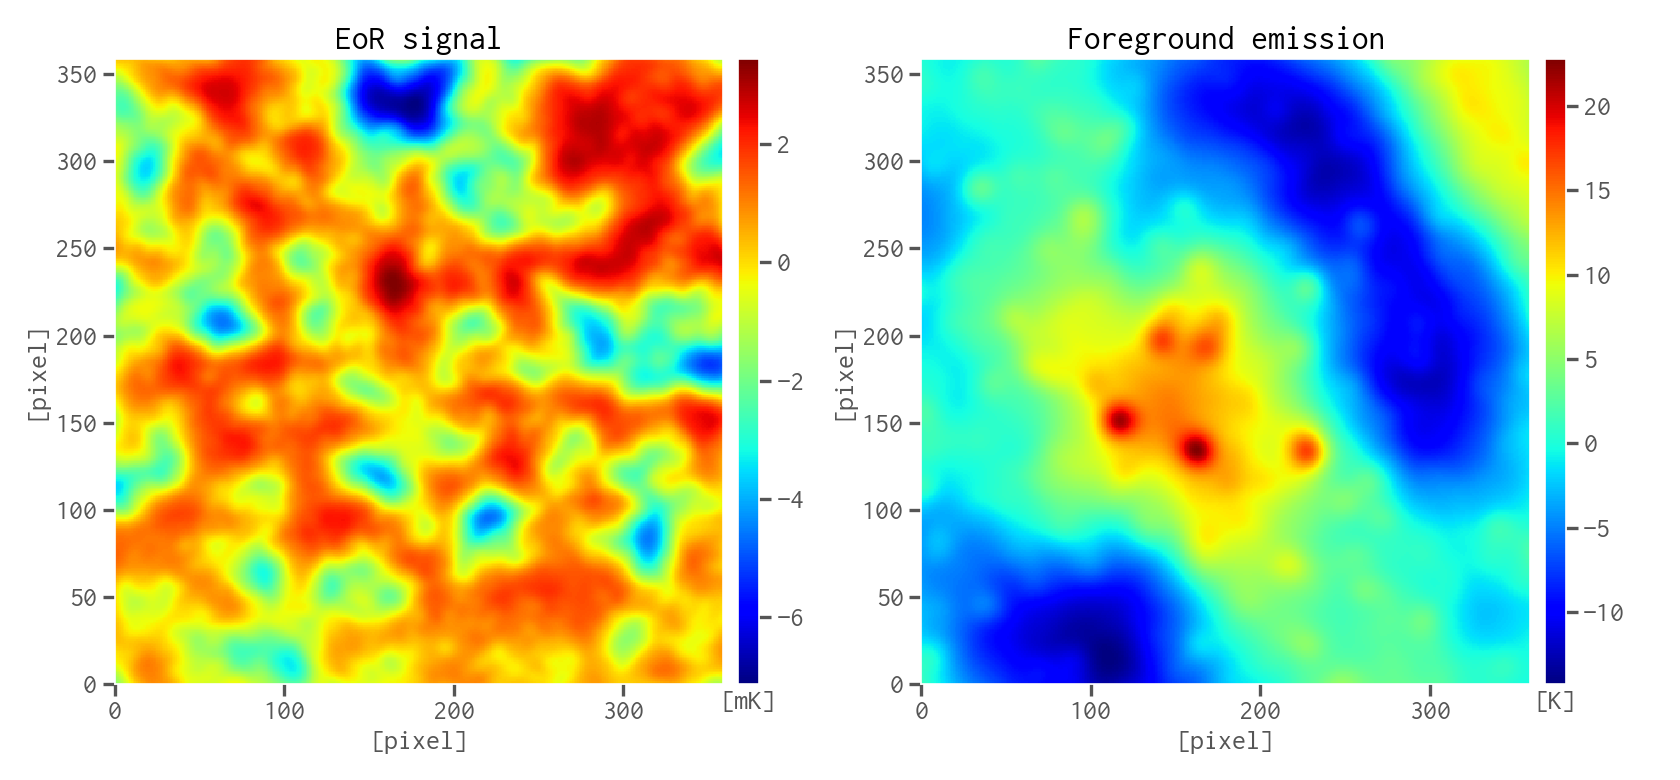
\includegraphics[width=\textwidth]{eor-fg-obsimg-158}
  \bicaption[EoR 信号和前景辐射在 \SI{158}{\MHz} 的模拟图像]{%
    EoR 信号(左栏)和前景辐射(右栏)在 \SI{158}{\MHz} 的模拟图像.
    两张图像的尺寸均为 \num{360 x 360} 并且覆盖天区的大小均为  \SI{2 x 2}{\degree}.
    右栏前景辐射图像中的斑点为明亮的点源和射电晕.
  }{%
    Simulated images of the EoR signal (left panel) and the foreground
    emission (right panel) at \SI{158}{\MHz}.
    Both images have sizes of \num{360 x 360} and cover sky areas of
    \SI{2 x 2}{\degree}.
    The blobs in the right panel show the bright point sources and radio
    halos.
  }
  \label{fig:eor-fg-obsimg}
\end{figure}

为了在模拟的\ac{skymap}中整合实际的波束效应,
我们按照 \autoref{sec:obs-simu} 所述方法对\ac{skymap}开展模拟观测,
获得了 SKA1-Low 的\enquote{观测}图像.
不过,我们根据这里的具体需求对 \autoref{sec:obs-simu} 的模拟方法进行了若干微调,
具体如下:
\begin{itemize}
  \item 因为我们只区分 EoR 信号和前景辐射,
    所以将所有前景成分的\ac{skymap}叠加起来再输入 \texttt{OSKAR} 模拟;
  \item 假定 \SI{158}{\MHz} 流量密度 $S_{158} > \SI{10}{\mJy}$
    的河外点源已被全部去除 \cite{liu2009ps};
  \item 为了强调暗弱而且比较弥散的 EoR 信号,
    我们在使用 \texttt{WSClean} 成像时选择了自然权重 (natural weighting),
    同时将基线范围限制在 \numrange{30}{1000} 个波长;
  \item 为了得到最佳的图像质量,我们只切取中央 \SI{2 x 2}{\degree}
    的区域,对应的图像尺寸为 \num{360 x 360}.
\end{itemize}
这样,我们得到了一对尺寸为 \num{360 x 360 x 101} 的\ac{imgcube}:
EoR 信号 $C_{\R{eor}}^{(1)}$ 和前景辐射 $C_{\R{fg}}^{(1)}$.
\autoref{fig:eor-fg-obsimg} 展示了两者在中心频率 \SI{158}{\MHz} 的模拟图像.

为了突出显示波束效应对前景辐射的频谱的影响,我们随机地选取一个天空像素点为例,
然后对比有无波束效应的情况下前景辐射的频谱变化,如\autoref{fig:cdae-simdata} 所示,
其中还显示了相应的差分频谱(即相邻两个频谱\ac{channel}的差值)以及 EoR 信号的频谱.
可以看出,前景辐射的本征频谱是非常光滑的(上栏),
但是在复杂的波束效应的影响下出现了许多小幅度、小尺度 (\SI{< 1}{\MHz}) 的涨落(中栏),
因此,频谱的光滑性受到了严重损坏.
尽管这些小尺度的涨落与 EoR 信号(下栏)具有一些相似的频谱特征,
但两者之间仍然具有足够的可区分度,可以被 \ac{cdae} 发掘出来并用于 EoR 信号的分离.
此外,\autoref{fig:cdae-simdata} 还显示出\enquote{观测}的前景辐射(中栏)
的强度相比原来的理想情况(上栏)约小 2 个数量级,
导致这个差异的主要原因是因为干涉阵列无法测量天空辐射的绝对强度,
只能响应辐射的空间涨落 \cite{braun1985}.

\begin{figure}[htp]
  \centering
  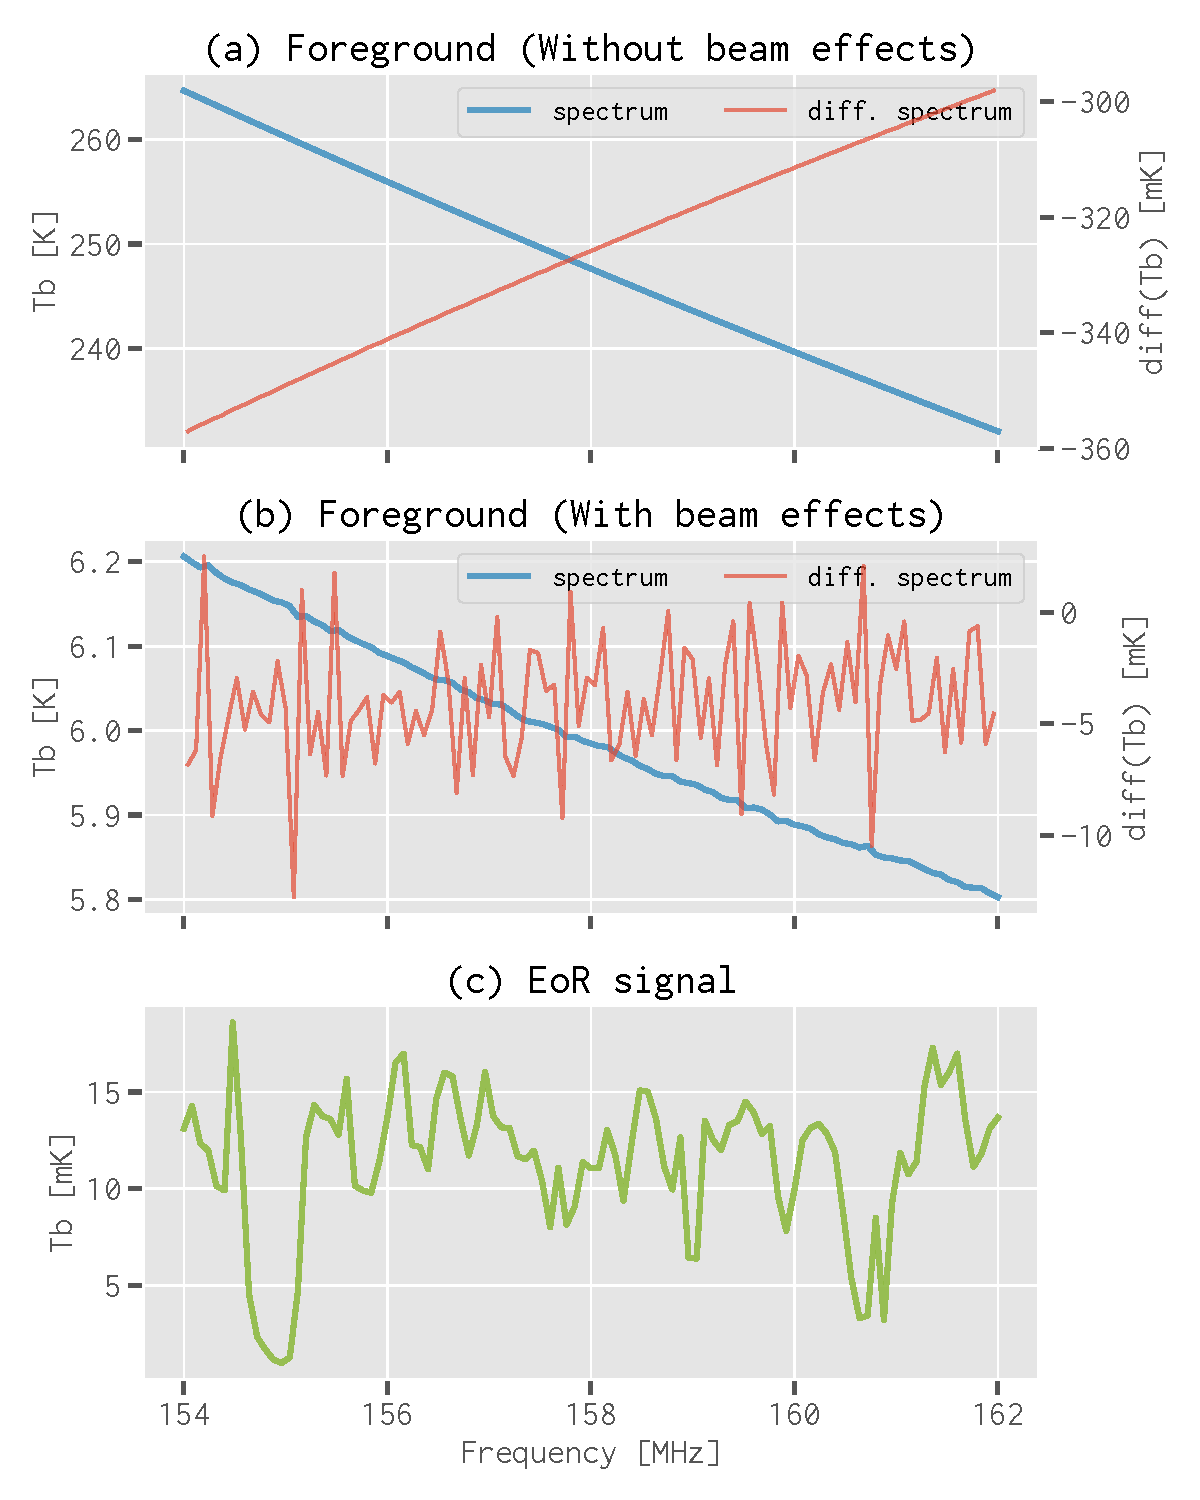
\includegraphics[width=0.85\textwidth]{cdae-simdata-example}
  \bicaption[前景辐射和 EoR 信号的频谱示例]{%
    随机取一个天空像素点为例,得到的前景辐射和 EoR 信号的频谱.
    \uline{(上栏)}
    理想的(即没有波束效应)前景辐射频谱(蓝线)以及相应的差分频谱(红线).
    \uline{(中栏)}
    仪器\enquote{观测}的(即包含波束效应)前景辐射频谱(蓝线)以及相应的差分频谱(红线).
    \uline{(下栏)}
    EoR 信号的频谱(绿线).
  }{%
    Example spectra of the foreground emission and the EoR signal for one
    random sky pixel.
    \emph{(Upper)} The ideal (i.e., without beam effects) foreground
    spectrum (blue line) and the corresponding differential spectrum
    (red line).
    \emph{(Middle)} The \enquote{observed} (i.e., with beam effects)
    foreground spectrum (blue line) and the corresponding
    differential spectrum (red line).
    \emph{(Lower)} The EoR signal spectrum (green line).
  }
  \label{fig:cdae-simdata}
\end{figure}

训练和评估 \ac{cdae} 需要三个\ac{ds},
分别为\acl{s-training}、\acl{s-validation} 和\acl{s-test}
(\autoref{sec:train-eval}),
如果只有一对\ac{imgcube},那么\acl{s-test} \ac{s-test} 只能包含一小部分的像素点的数据,
而且这些像素点随机地分布在天空平面里.
在 \ac{cdae} 的测试阶段 (\autoref{sec:cdae-results}),
利用这样一个\acl{s-test} \ac{s-test} 重建得到的 EoR 信号无法构成完整的
(甚至局部完整的)\ac{imgcube},
从而无法通过图像和\ac{ps}直观地展示 \ac{cdae} 分离 EoR 信号的效果.
因此,为\acl{s-test} \ac{s-test} 再额外模拟一对\ac{imgcube}能够解决上述问题.
由于最终经过切取的\ac{imgcube}所覆盖的天区大小仅有 \SI{2 x 2}{\degree},
我们设第二对\ac{imgcube}的中心坐标为
(R.A., Dec.\@) = (\SI{3}{\degree}, \SI{-27}{\degree}),
即与第一对\ac{imgcube}
$\left( C_{\R{eor}}^{(1)}, C_{\R{fg}}^{(1)} \right)$
的中心相距 \SI{3}{\degree}.
具体而言,我们以 (R.A., Dec.\@) = (\SI{3}{\degree}, \SI{-27}{\degree})
为中心模拟了银河系弥散辐射(\ac{rad-syn}和\ac{rad-ff})的\ac{skymap};
因为河外点源、射电晕以及 EoR 信号的空间分布几乎是各向同性的,
所以我们将它们原来的\ac{skymap}平移 \SI{3}{\degree} 得到所需的新\ac{skymap}.
然后,遵循相同的模拟观测方法,我们得到了第二对\ac{imgcube}
$\left( C_{\R{eor}}^{(2)}, C_{\R{fg}}^{(2)} \right)$.

鉴于我们所提出的新算法适用于 EoR \ac{tomography},
要求极深度的观测以达到足够低的噪声水平.
比如,SKA1-Low 计划筛选 5 个 EoR 天区,然后对每个天区观测约 \SI{1000}{\hour},
达到空前的约小于 \SI{1}{\mK} 的亮度灵敏度 [\autoref{eq:sigma-tb}],
从而实现 EoR 区域的直接成像观测 \cite{mellema2013,mellema2015,koopmans2015}.
因此,我们没有在上述模拟中包含仪器的热噪声.

%---------------------------------------------------------------------
\subsection{数据预处理}
\label{sec:preprocessing}

按照天空像素点将 \autoref{sec:cdae-images} 模拟得到的\ac{imgcube}重新组织,
形成一系列数据点 $\left( \B{x}^{(i)}, \,\B{x}^{(i)}_{\R{eor}} \right)$,
其中 $\B{x}^{(i)}_{\R{eor}}$ 和
$\B{x}^{(i)} = \B{x}^{(i)}_{\R{eor}} + \B{x}^{(i)}_{\R{fg}}$
分别表示像素点 $i$ 的 EoR 信号和总辐射的频谱.
数据点的总数为 $N_S = \num{360x360 x 2} = \num{259200}$,
这些数据点组成了训练和评估 \ac{cdae} 所需的\ac{ds}
$S = \left\{ \left(\B{x}^{(i)}, \,\B{x}^{(i)}_{\R{eor}} \right) \right\}$.
但是,\ac{cdae} 在使用该数据集 $S$ 时,
需要分别对输入的总辐射 $X = \big\{ \B{x}^{(i)} \big\}$
以及 EoR 信号 $X_{\R{eor}} = \big\{ \B{x}^{(i)}_{\R{eor}} \big\}$
进行合适的预处理.

对于输入数据 $X = \big\{ \B{x}^{(i)} \big\}$,
我们提出首先对信号 $\B{x}^{(i)}$ 进行 Fourier 变换.
这样可以提高 EoR 信号与前景辐射之间的可分度,
于是 \ac{cdae} 能够更容易、更好地学习两者之间的差异.
(我们将在 \autoref{sec:why-ft} 讨论不使用 Fourier 变换预处理数据时所得到的结果.)
由于信号 $\B{x}^{(i)}$ 的长度为 $n_f = 101$ 是有限的,
为了抑制信号的边界效应使 Fourier 变换产生显著的\ac{sidelobe}
(\autoref{sec:eval-method}),
我们在 Fourier 变换前对信号 $\B{x}^{(i)}$ 施加 Blackman--Nuttall \ac{f-window}
\cite{chapman2016} [\autoref{eq:bn-window}].
因为信号 $\B{x}^{(i)}$ 全部由实数组成,
所以变换后的 Fourier 系数 $\hat{x}^{(i)}_{f}$ 具有以下对称关系:
\begin{equation}
  \hat{x}^{(i)}_{f} \equiv \hat{x}^{*(i)}_{-f} ,
\end{equation}
其中 $f$ 表示 Fourier 频率,\enquote{$*$} 为\ac{conjugate}算符.
因此,只需要保留一半的 Fourier 系数即可.
于是,长度为 $n_f = 101$ 的信号 $\B{x}^{(i)}$ 变换为
$n_c = 51$ 个复 Fourier 系数:
\begin{equation}
  \left( \hat{x}^{(i)}_f; \; f = 0, 1, \cdots, 50 \right) ,
\end{equation}
其中,Fourier 频率 $f$ 最小的几个系数主要由频谱光滑的前景辐射贡献,
因此可以通过排除这几个 Fourier 系数来抑制前景干扰.
为了平衡前景辐射的抑制效果和 EoR 信号的损失程度,
经过测试,我们选择排除 $n_{\R{ex}} = 6$ 个 Fourier 频率最小的系数,
于是剩下的 45 个 Fourier 系数为:
\begin{equation}
  \left( \hat{x}^{(i)}_f; \; f = 6, 7, \cdots, 50 \right) .
\end{equation}
因为 \ac{cdae} 只能处理实数,
所以我们将这些复 Fourier 系数的实部和虚部分开,
设 $\hat{x}^{(i)}_f = a_f + \Ci\,b_f$,
然后重新拼接成一个长度为 $n_d = 90$ 的实矢量:
\begin{equation}
  (a_6, a_7, \cdots, a_{49}, a_{50},
   b_{50}, b_{49}, \cdots, b_7, b_6) .
\end{equation}
最后,将数据标准化,使其平均值为 0、标准差为 1.

对于输入的 EoR 信号 $X_{\R{eor}} = \big\{ \B{x}^{(i)}_{\R{eor}} \big\}$,
我们首先使用与上述 $X$ 相同的预处理方法:
进行 Fourier 变换,接着去除 $n_{\R{ex}}$ 个 Fourier 频率最小的系数,
再将复 Fourier 系数的实部和虚部拼接成实矢量.
后续的预处理步骤则与 $X$ 的预处理方法有所不同.
计算数据的第 1 和第 99 \ac{percentile},
然后将小于第 1 \ac{percentile}以及大于第 99 \ac{percentile}的元素截断,
用来防止数据中可能存在的\ac{outlier}阻碍 \ac{cdae} 的训练.
最后,将数据除以其最大绝对值,使其数值范围为 $[-1, 1]$.
这种处理方法允许我们在 \ac{cdae} 的输出层使用值域同样为 $[-1, 1]$
的 \enquote{tanh} 函数作为\ac{f-activation} (\autoref{sec:architecture}).

%---------------------------------------------------------------------
\subsection{训练和结果}
\label{sec:cdae-results}

The preprocessed data of the first cube pair
$\left( C_{\R{eor}}^{(1)}, C_{\R{fg}}^{(1)} \right)$
are randomly partitioned into the training set ($S_{\R{tr}}$; corresponding
to 80 per cent of the pixels, or \num{103680} data points) and the
validation set ($S_{\R{val}}$; 20 per cent, or \num{25920} data points).
The preprocessed data of the second cube pair
$\left( C_{\R{eor}}^{(2)}, C_{\R{fg}}^{(2)} \right)$
are solely used as the test set ($S_{\R{test}}$; \num{129600} data points).
The use of the whole image cubes as the test set enables us to create
complete images of the reconstructed EoR signal.

We implement the proposed CDAE using the
\href{https://keras.io}{\texttt{Keras}}\footnote{%
  Keras: \url{https://keras.io} (v2.2.4)}
framework \cite{keras} with the
\href{https://www.tensorflow.org}{\texttt{TensorFlow}}\footnote{%
  TensorFlow: \url{https://www.tensorflow.org} (v1.12.0)}
back end \cite{tensorflow},
which is accelerated by the
\href{https://developer.nvidia.com/cuda-zone}{\texttt{CUDA}}\footnote{%
  CUDA: \url{https://developer.nvidia.com/cuda-zone} (v9.1.85)}
toolkit.
We adopt a small initial learning rate ($\alpha = \num{e-5}$) and use the
Adam optimisation method \cite{kingma2015}.
The CDAE is trained on the training set ($S_{\R{tr}}$) with a batch size of
100 until the training loss converges, which takes about 50 epochs.

\begin{figure}[htp]
  \centering
  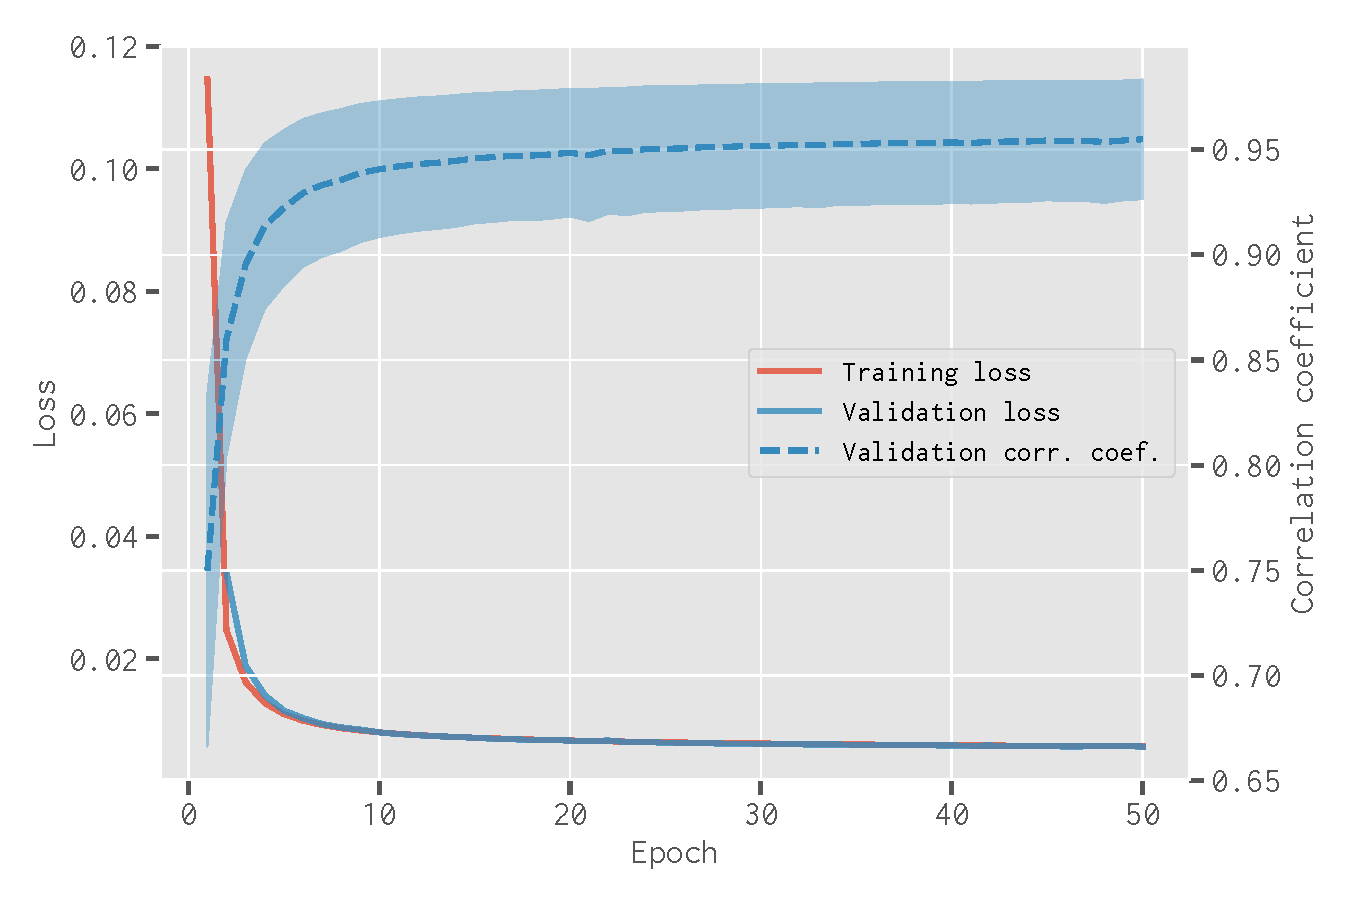
\includegraphics[width=\textwidth]{cdae-train}
  \bicaption[训练 CDAE 的过程和结果]{%
    TODO...
  }{%
    The training loss (solid red line), validation loss (solid blue
    line), and correlation coefficient ($\rho$; dashed blue
    line with the shaded region representing its standard deviation)
    calculated on the validation set $S_{\R{val}}$ along the training of
    the CDAE.
  }
  \label{fig:cdae-train}
\end{figure}

\begin{figure}[htp]
  \centering
  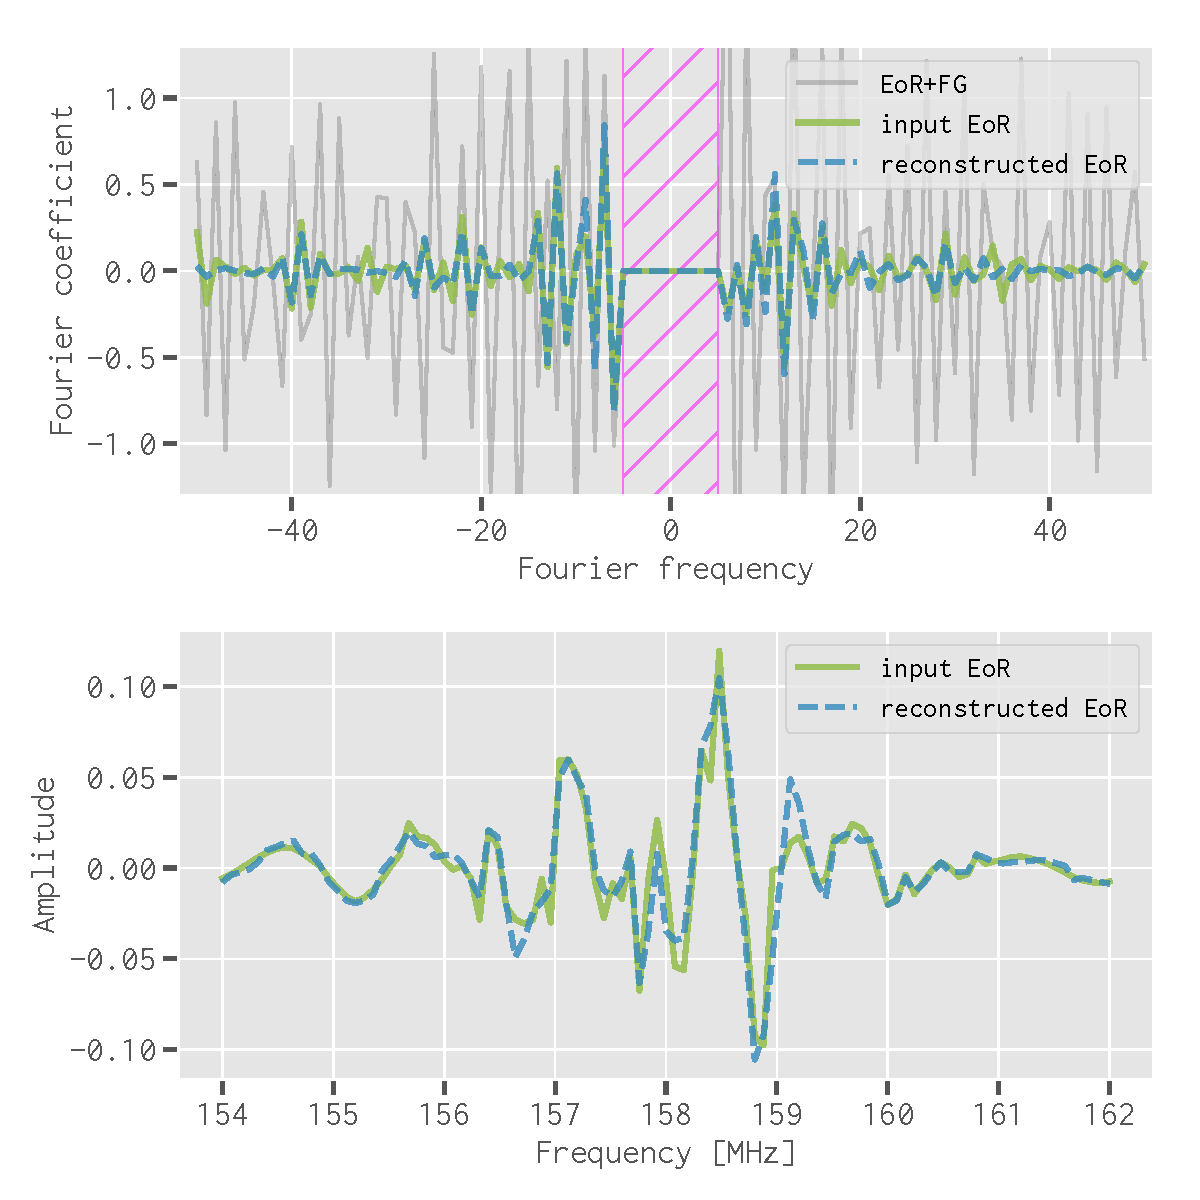
\includegraphics[width=\textwidth]{cdae-eor-pix}
  \bicaption[CDAE 重建的 EoR 信号的示例]{%
    TODO...
  }{%
    An example of the EoR signal reconstructed by the trained CDAE for
    one pixel in $S_{\R{test}}$.
    \textbf{(top)} The input EoR signal $\B{x}_{\R{eor}}$ (solid
    green line) and the reconstructed EoR signal $\B{r}_{\R{eor}}$
    (dashed blue line) in the Fourier domain.
    The correlation coefficient between the input and
    reconstructed EoR signals is $\rho = 0.931$.
    The gray line represents the input total emission
    $\B{x} = \B{x}_{\R{fg}} + \B{x}_{\R{eor}}$.
    The magenta hatched region marks the excised Fourier coefficients
    in data preprocessing.
    \textbf{(bottom)} The input EoR signal $\B{x}_{\R{eor}}$ (solid
    green line) and the reconstructed EoR signal $\B{r}_{\R{eor}}$
    (dashed blue line) transformed back to the observing frequency
    domain.
  }
  \label{fig:cdae-eor-pix}
\end{figure}

The training and validation losses together with the evaluation index
(i.e., the correlation coefficient $\rho$) calculated on the validation set
$S_{\R{val}}$ during the training phase are shown in \autoref{fig:cdae-train}.
The steadily decreasing losses and increasing correlation coefficient
suggest that the CDAE is well trained without over-fitting.
After training, the evaluation with the test set $S_{\R{test}}$ yields a
high correlation coefficient of $\bar{\rho}_{\R{cdae}} = \num{0.929 +- 0.045}$
between the reconstructed and input EoR signals.
This result demonstrates
that the trained CDAE achieves excellent performance in reconstructing the
EoR signal.
As an example, \autoref{fig:cdae-eor-pix} illustrates the reconstructed EoR
signal ($\rho = 0.931$) for one pixel in $S_{\R{test}}$.

\begin{figure}[htp]
  \centering
  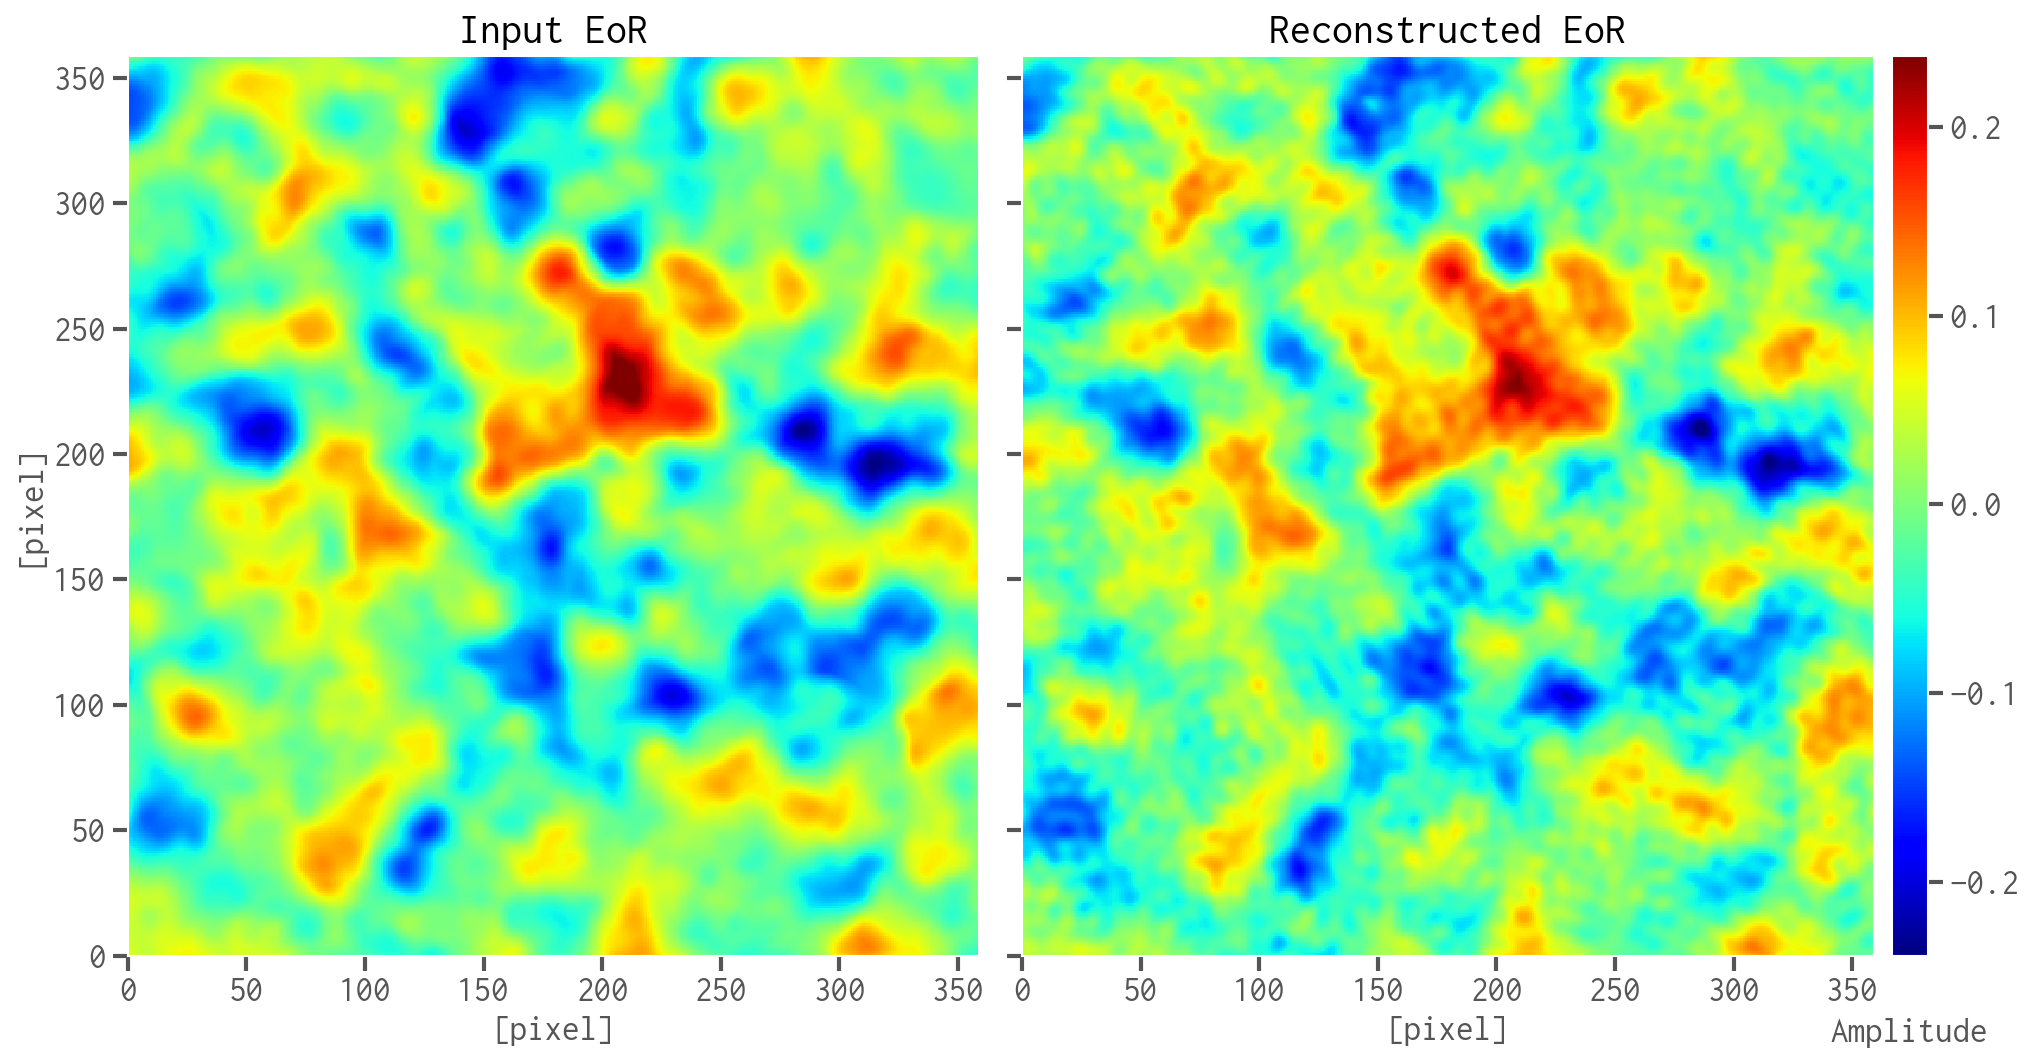
\includegraphics[width=\textwidth]{cdae-eor-img-comp}
  \bicaption[输入的 EoR 图像和 CDAE 重建的 EoR 图像的对比]{%
    TODO...
  }{%
    Comparison between the input EoR image (the left panel) and
    reconstructed EoR image (the right panel) at the central frequency of
    \SI{158}{\MHz}.
    The images have the same size (\num{360 x 360} pixel) and the figures
    share the same color bar (the amplitude is normalized for the CDAE).
  }
  \label{fig:cdae-eor-img}
\end{figure}

\begin{figure}[htp]
  \centering
  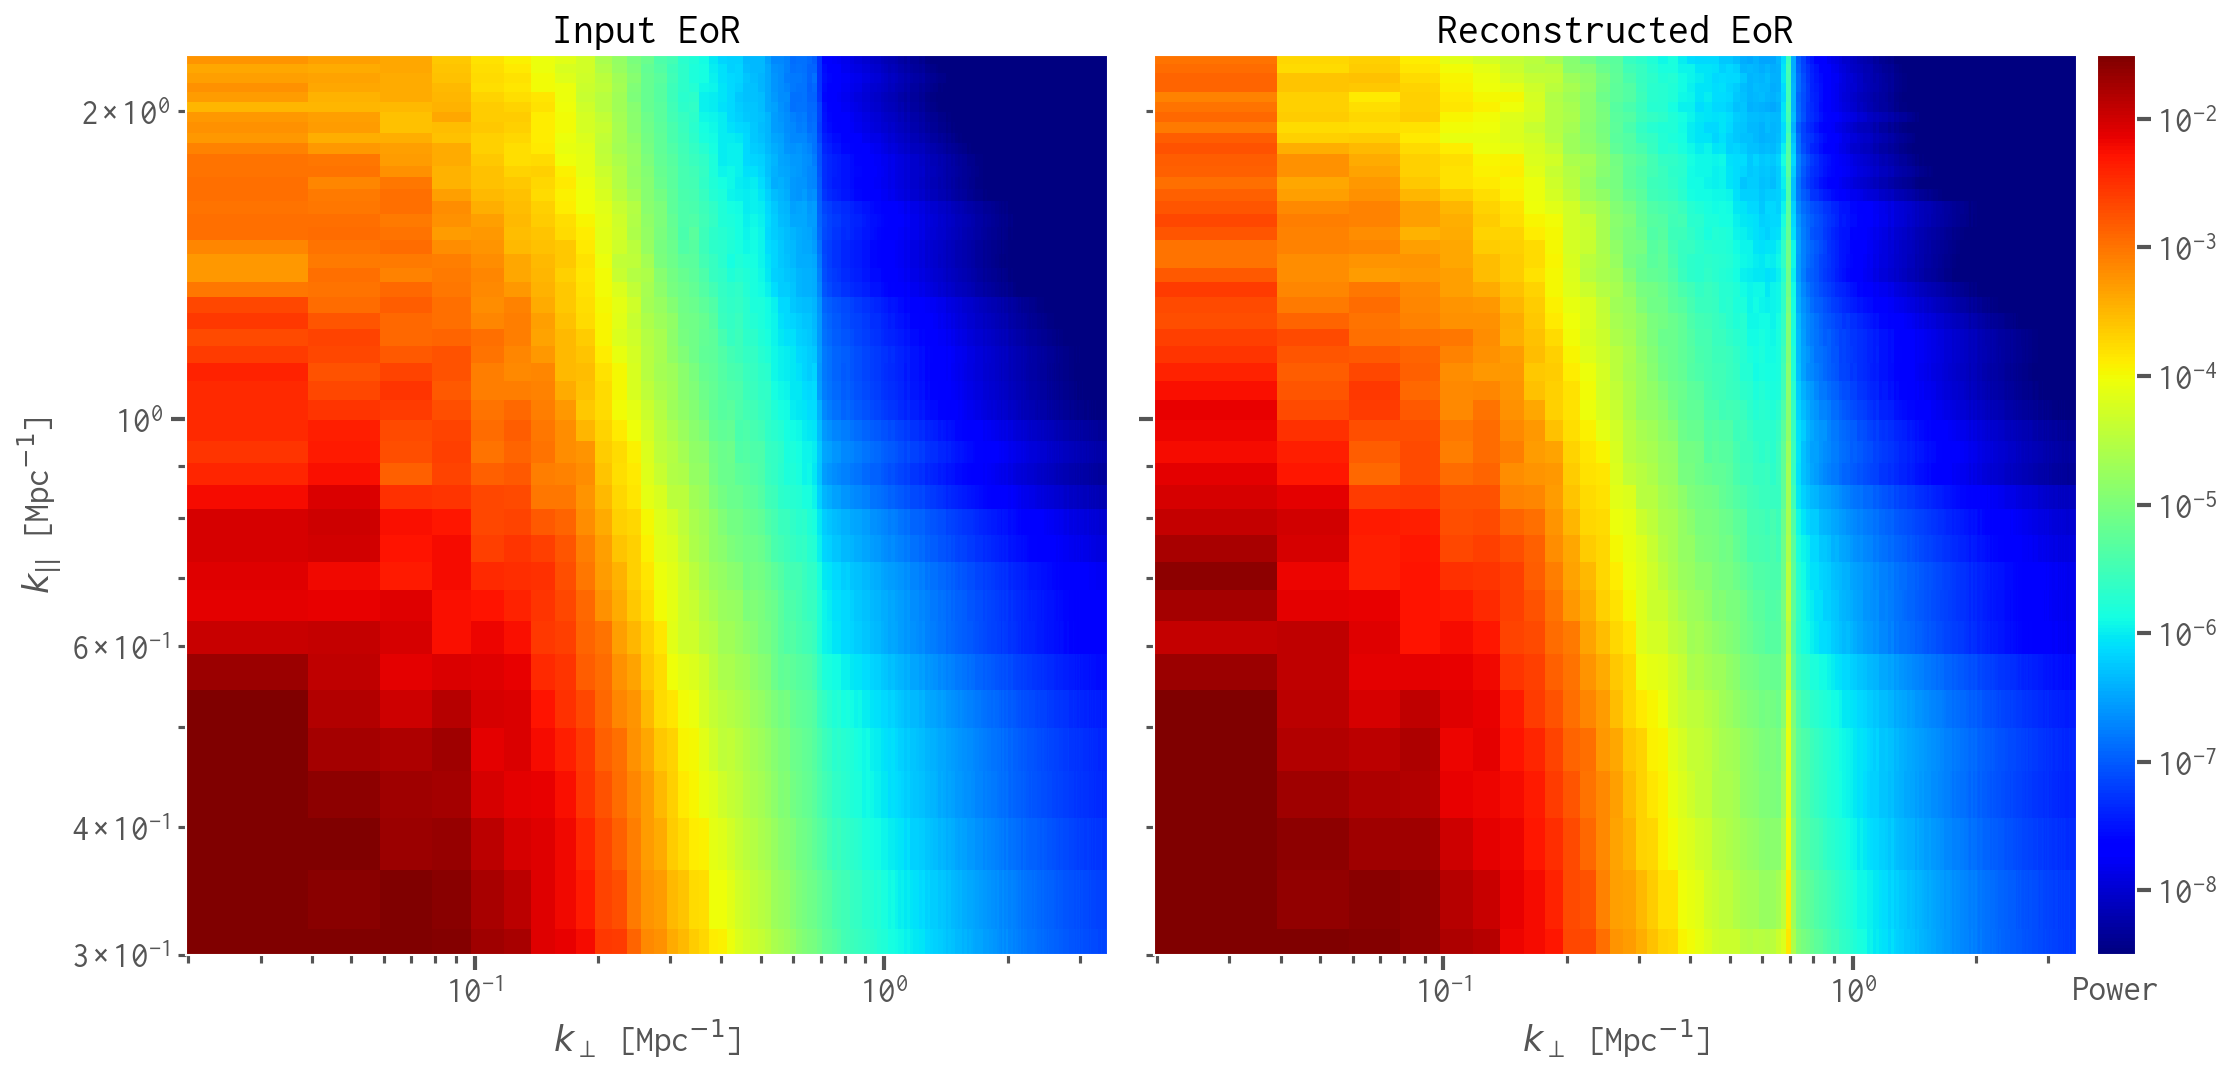
\includegraphics[width=\textwidth]{cdae-eor-ps-comp}
  \bicaption[输入的 EoR 信号和 CDAE 重建的 EoR 信号之间的二维功率谱对比]{%
    TODO...
  }{%
    Comparison of two-dimensional power spectra between the input (the left
    panel) and reconstructed (the right panel) EoR signals.
  }
  \label{fig:cdae-eor-ps}
\end{figure}

Since the test set $S_{\R{test}}$ is derived from the whole image cubes
$\left( C_{\R{eor}}^{(2)}, C_{\R{fg}}^{(2)} \right)$, we are able to create
complete images of the reconstructed EoR signal and calculate the
corresponding power spectrum.
Taking the input and reconstructed EoR images at the central frequency of
\SI{158}{\MHz} as an example (\autoref{fig:cdae-eor-img}), the reconstructed EoR
signal exhibits almost identical structures and amplitudes as the input EoR
signal.
We note that the reconstructed EoR image has weak but detectable redundant
ripples on scales of about 10 pixels (i.e., \SI{\sim 200}{\arcsecond}),
which are associated with the excision of the $n_{\R{ex}} = 6$ lowest
Fourier frequencies in data preprocessing (\autoref{sec:preprocessing}).
In addition, we calculate the two-dimensional power spectra from the image
cubes of the input and reconstructed EoR signals (\autoref{fig:cdae-eor-ps}).
It illustrates that the trained CDAE well recovers the EoR signal on all
covered scales except for a very thin stripe region at
$\kperp \approx \SI{0.7}{\per\Mpc}$, where extra powers are generated
by the aforementioned ripples in the reconstructed EoR images.
We also note that there is a barely visible line at
$\kperp \approx \SI{0.1}{\per\Mpc}$ in both power spectra, which is
caused by the boundary effect of Fourier transforming the finite frequency
band.

The results clearly demonstrate that the trained CDAE is able to accurately
reconstruct the EoR signal, overcoming the complicated beam effects.
The achieved excellent performance of the CDAE can be mainly attributed
to the architecture of stacking multiple convolutional layers, which
implements a powerful feature extraction technique by hierarchically
combining the basic features learned in each layer to build more and
more sophisticated features \cite{leCun2015}.
Combined with the flexibility provided by the \num{53569} trainable
parameters, the CDAE, after being well trained, can intelligently learn a
model that is optimised to accurately separate the faint EoR signal
\cite{domingos2012}.

%---------------------------------------------------------------------
\subsection{进一步验证}
\label{sec:cdae-validation}

With the purpose of further validating that the trained CDAE has actually
learned the useful features of the EoR signal, we employ the occlusion
method \cite{zeiler2014} to visualise the sensitivity of the trained CDAE
to the different part of the input data.
At each time, we occlude three adjacent elements of every input
$\B{x}$ in the validation set $S_{\R{val}}$, and then measure the CDAE's
sensitivity to the occluded part, which is calculated as the
occlusion-induced performance loss, i.e.,
\begin{equation}
  \label{eq:perf-loss}
  s = \frac{1}{N_{\R{val}}} \sum_{i=1}^{N_{\R{val}}} \left[
      \rho\left(\B{r}^{(i)}_{\R{eor}}, \B{x}^{(i)}_{\R{eor}}\right) -
      \rho\left(\B{R}^{(i)}_{\R{eor}}, \B{x}^{(i)}_{\R{eor}}\right)
    \right] ,
\end{equation}
where
$N_{\R{val}}$ is the number of data points in the validation set,
$\B{x}^{(i)}_{\R{eor}}$ is the input EoR signal, and
$\B{r}^{(i)}_{\R{eor}}$ and $\B{R}^{(i)}_{\R{eor}}$ are the reconstructed
EoR signals without and with applying the occlusion, respectively.
By varying the occlusion part of the input data and calculating the
sensitivities, we obtain the CDAE's sensitivity distribution ($\B{s}$) to
every part of the input data, as shown in \autoref{fig:occ-fgeor}, where
the root-mean-square amplitudes of the foreground emission
($\B{y}_{\R{fg}}$) and the EoR signal ($\B{y}_{\R{eor}}$) are also plotted.
We find that the sensitivity distribution is more correlated with the EoR
signal [$\rho(\B{s}, \B{y}_{\R{eor}}) = 0.742$] than the foreground
[$\rho(\B{s}, \B{y}_{\R{fg}}) = 0.562$].
This verifies that the trained CDAE has learned useful features of the EoR
signal to distinguish it from the foreground emission and thus becomes more
sensitive to the data parts of higher signal-to-noise ratio.

\begin{figure}[htp]
  \centering
  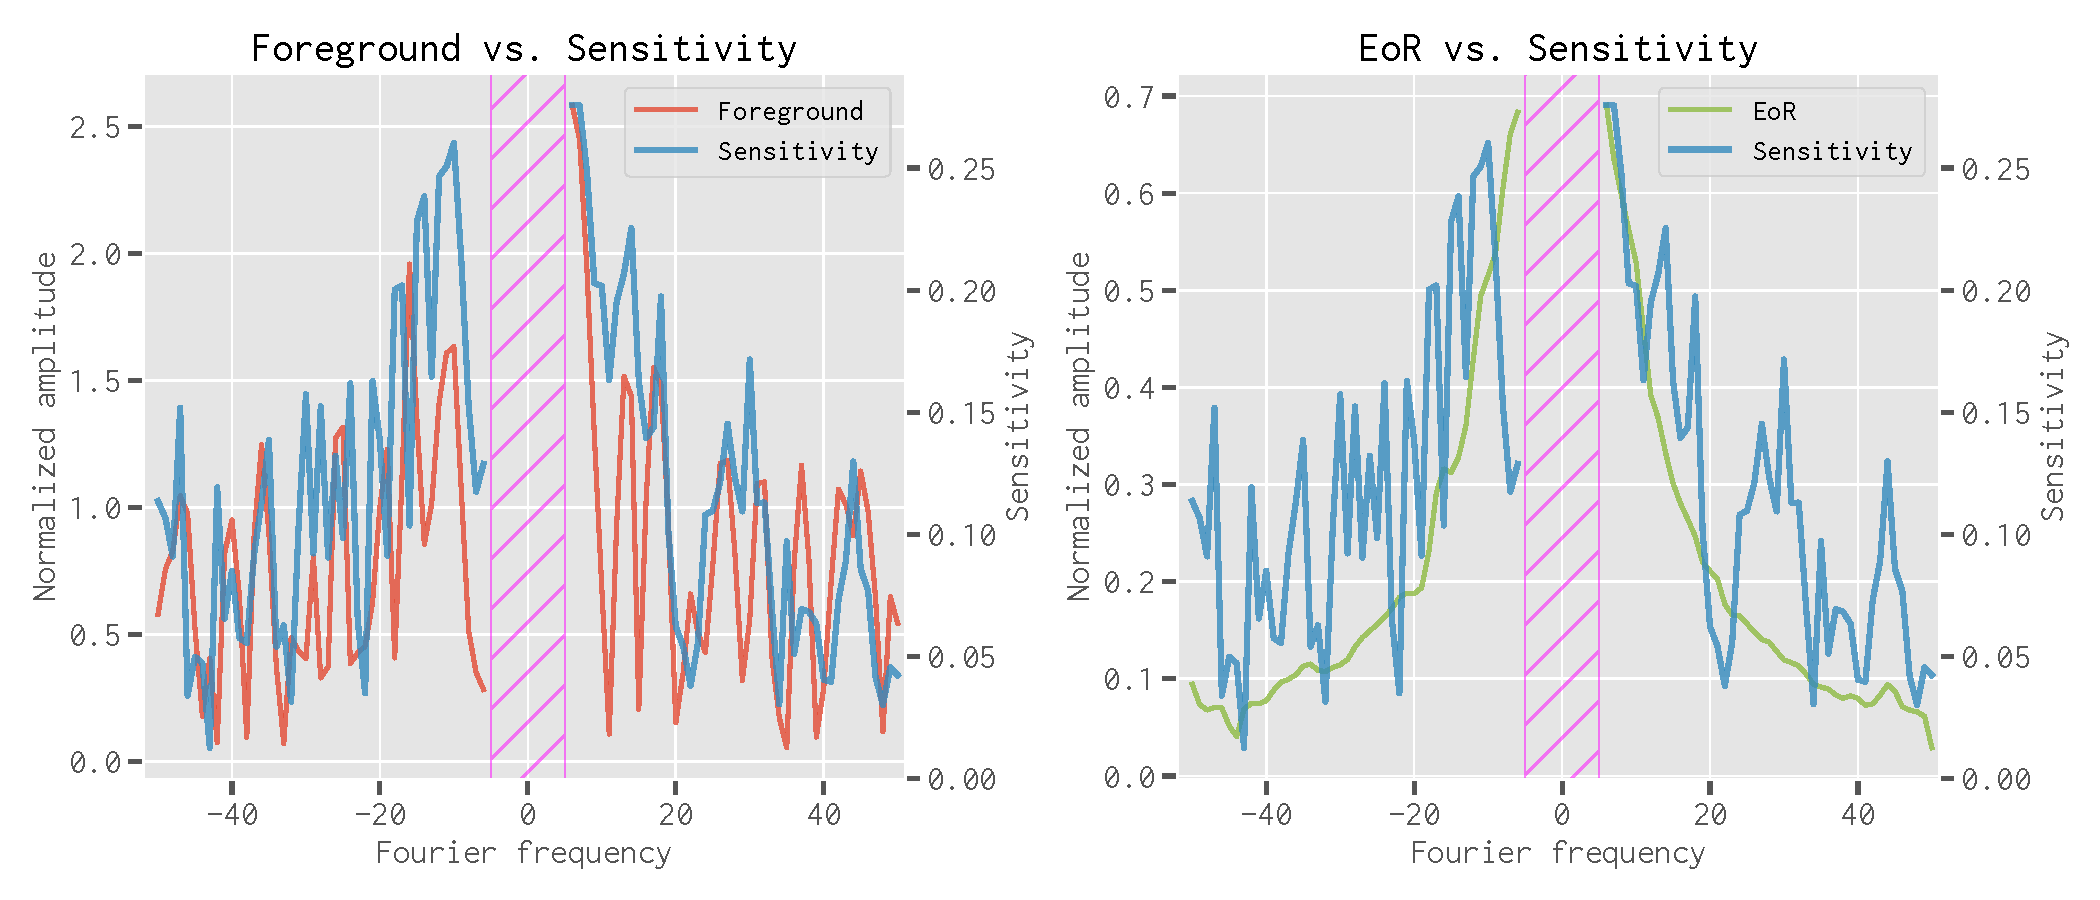
\includegraphics[width=\textwidth]{occlusion-fgeor}
  \bicaption[CDAE 对输入数据的灵敏度分布]{%
    TODO...
  }{%
    The CDAE's sensitivity distribution $\B{s}$ (the blue lines in both
    panels) obtained by applying the occlusion method.
    We also plot the root-mean-square amplitudes of the foreground emission
    ($\B{y}_{\R{fg}}$, the red line in the left panel) and the EoR signal
    ($\B{y}_{\R{eor}}$, the green line in the right panel).
    The sensitivity distribution $\B{s}$ is more correlated with the EoR
    signal [$\rho(\B{s}, \B{y}_{\R{eor}}) = 0.742$] than the foreground
    [$\rho(\B{s}, \B{y}_{\R{fg}}) = 0.562$].
  }
  \label{fig:occ-fgeor}
\end{figure}


%=====================================================================
\section{讨论}

TODO

%---------------------------------------------------------------------
\subsection{为什么使用 Fourier 变换预处理数据?}
\label{sec:why-ft}

We perform another experiment using the same CDAE architecture,
datasets, and data preprocessing steps, but without
applying the FT as depicted in \autoref{sec:preprocessing}.
After training the CDAE in the same way as described in
\autoref{sec:cdae-results}, the correlation coefficient between the
reconstructed and input EoR signals evaluated on the test set
$S_{\R{test}}$ reaches only $\bar{\rho}_{\R{noft}} = \num{0.628 +- 0.167}$,
which indicates a significantly worse performance compared to the case with
FT applied.
As presented in \autoref{fig:cdae-train-noft}, the training loss decreases more
slowly and converges after about 100 epochs.
We also find that the training process is slightly unstable given the small
spikes on the curves of both the loss and correlation coefficient.
These indicate that it is beneficial to preprocess the
dataset by applying the FT along the frequency dimension, because the
EoR signal and the foreground emission become more distinguishable
in the Fourier domain, where the fluctuating EoR signal concentrates on
larger Fourier modes while the spectral-smooth foreground emission
distributes mainly on smaller Fourier modes \cite{parsons2012}.

\begin{figure}[htp]
  \centering
  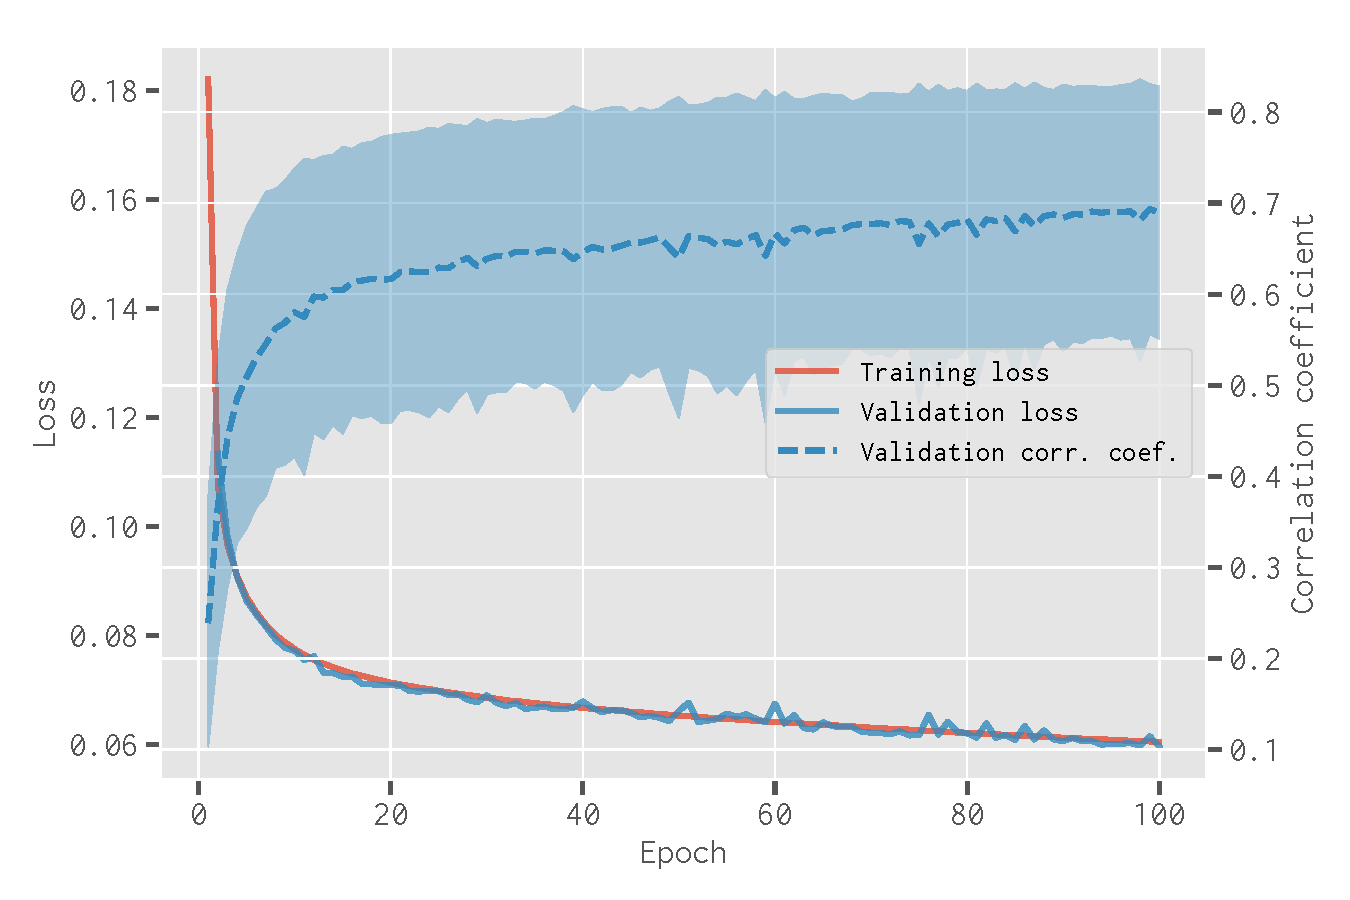
\includegraphics[width=\textwidth]{cdae-train-noft}
  \bicaption[在未经 Fourier 变换预处理的数据集上训练 CDAE 得到的结果]{%
    TODO... \autoref{fig:cdae-train}
  }{%
    Same as Fig.~\ref{fig:cdae-train} but for the case that the data are
    preprocessed without applying the FT.
  }
  \label{fig:cdae-train-noft}
\end{figure}


%---------------------------------------------------------------------
\subsection{与传统方法的对比}

A variety of methods have been proposed to remove the foreground
contamination with the aim of revealing the faint EoR signal.
These methods can be broadly classified into two categories:
(1) parametric methods that apply a parametric model (e.g., a low-degree
polynomial) to fit and remove the foreground emission
\cite{wang2006,jelic2008,liu2009fgrm,wang2013,bonaldi2015};
(2) non-parametric methods, which do not assume a specific parametric model
for the foreground emission but exploit the differences between the
foreground emission and the EoR signal (e.g., their different spectral
features) to separate them
\cite{harker2009,chapman2012,chapman2013,gu2013,mertens2018}.

In order to further demonstrate the performance of our method, we compare
it to two representative traditional methods:
the polynomial fitting method \cite{wang2006} and
the continuous wavelet transform (CWT) method \cite{gu2013}.
The polynomial fitting method is the best representative of the parametric
methods because it is widely used due to its simplicity and robustness
\cite{jelic2008,liu2009ps,pritchard2010}
and has been compared to various other foreground removal methods
\cite{harker2009,alonso2015,chapman2015}.
Among the non-parametric category, the CWT method is chosen since it
performs similarly well as other non-parametric methods, such as the
Wp smoothing method \cite{harker2009} and the generalized morphological
component analysis method \cite{chapman2013},
meanwhile it is faster and simpler \cite{gu2013,chapman2015}.

With the polynomial fitting method,
a low-degree polynomial is fitted along the frequency dimension for each
sky pixel in the image cube of the total emission (i.e.,
$C_{\R{tot}} = C_{\R{eor}} + C_{\R{fg}}$).
Then by subtracting the fitted smooth component, which is regarded as
the foreground emission, the EoR signal is expected to be uncovered.
Using the same image cubes
$\left( C_{\R{eor}}^{(2)}, C_{\R{fg}}^{(2)} \right)$
simulated in \autoref{sec:cdae-images},
we have tested polynomials of the degree from 2 (quadratic) to
5 (quintic), and find that the quartic polynomial (degree of 4)
can give the best result.
However, the correlation coefficient calculated for the separated EoR
signal in such a case is only
$\bar{\rho}_{\R{poly}} = \num{0.296 +- 0.121}$,
which indicates that the polynomial fitting method performs poorly in
removing the foreground emission.

The CWT method works based on the same assumption as other foreground
removal methods that the foreground emission is spectrally smooth while the
EoR signal fluctuates rapidly along the frequency dimension.
After applying the CWT, the foreground emission and the EoR signal locate
at different positions in the wavelet space because of their different
spectral scales.
Therefore, the foreground emission can be easily separated from the EoR
signal and be removed \cite{gu2013}.
For each sky pixel, the spectrum of the total emission is transformed into
the wavelet space by applying the CWT with the Morlet wavelet function.
In the wavelet space, after identifying and removing the coefficients that
are mainly contributed by the foreground emission, the remaining
coefficients are transformed back to the frequency space to obtain the
spectrum with the foreground emission removed, which is expected to be the
EoR signal.
By evaluating on the same dataset
$\left( C_{\R{eor}}^{(2)}, C_{\R{fg}}^{(2)} \right)$,
we have tuned the method parameters (minimum scale $s_{\R{min}}$, maximum
scale $s_{\R{max}}$, number of scales $n_s$, and cone of influence $c_i$)
and adopt $s_{\R{min}} = 7.4$, $s_{\R{max}} = 50.0$, $n_s = 50$, and
$c_i = 1.6$ to obtain the relatively best performance, which is, however,
only $\bar{\rho}_{\R{cwt}} = \num{0.198 +- 0.160}$.
We note that the CWT method performs slightly worse than the polynomial
fitting method, which is different from the comparison in \citet{gu2013}.
This may be caused by the more serious boundary effect since our simulated
data have a narrower bandwidth and coarser frequency resolution than those
of \citet{gu2013}.

The main reason that both traditional foreground removal methods only
obtain remarkably inferior results is that the smoothness of the foreground
spectra is seriously damaged by the frequency-dependent beam effects, which
cause rapid fluctuations of strength the same order as the EoR signal on
the originally smooth foreground spectra [\autoref{fig:cdae-simdata}(b)].
As a result, the foreground spectra complicated by the beam effects cannot
be well fitted by a low-degree polynomial and have more similar spectral
scales as the EoR signal.
In consequence, both methods are unable to well model the complicated
foreground spectra and thus have great difficulties in removing them.
On the contrary, given its data-driven nature and powerful feature
extraction capabilities, the CDAE is able to distil knowledge from the
training data and learns the features to distinguish the EoR signal from
the fluctuations arising from the beam effects.
Hence, the CDAE achieves superior performance in separating the EoR signal.


%=====================================================================
\section{小结}

The frequency-dependent beam effects of interferometers can cause
rapid fluctuations along the frequency dimension,
which damage the smoothness of the foreground spectra and prevent
traditional foreground removal methods from uncovering the EoR signal.
Given the difficulties in crafting practicable models to overcome the
complicated beam effects, methods that can intelligently learn tailored
models from the data seem more feasible and appealing.
To this end, we have proposed a deep-learning-based method that uses
a 9-layer CDAE to separate the EoR signal.
The CDAE has been trained on the simulated SKA images and has achieved
excellent performance.
We conclude that the CDAE has outstanding ability to overcome the
complicated beam effects and accurately separate the faint EoR signal,
exhibiting the great potential of deep-learning-based methods
to play an important role in the forthcoming EoR experiments.

本章内容已发表于 \mnras{} (MNRAS)\reviewornot{}{\cite{li.cdae}}.


%% EOF
